\documentclass[a4paper,12pt]{report}
\usepackage[utf8]{inputenc}

\usepackage{hyperref}
\usepackage{cite}
\usepackage{algorithm}
\usepackage{algpseudocode}
\usepackage{graphicx}

\setlength\fboxsep{0pt}
\setlength\fboxrule{0.5pt}

\setcounter{secnumdepth}{5}

\DeclareGraphicsExtensions{.pdf,.png,.jpg}
%\usepackage{cleveref}

%%%%% definition of custom commands %%%%%

% use when you need a ref to a section with hyperlinks like: ``section x, Section Name''

\newcommand{\secref}[1]{\autoref{#1}, \nameref{#1}}
\newcommand{\And}{\textbf{ and }}
%\newcommand{\secref}[1]{\ref{#1}}

%%%%% end definition of custom commands %%%%%

%opening
\title{Rapid Geologic Modeling}
\author{Morten Bendiksen}

\begin{document}

\maketitle


\clearpage
\begin{abstract}
Drawing three dimentional models of geological phenomena is today a process requiring training in specific programs, and can be a time consuming process. For illustration and communication, geologists therefore often limit themselves to drawing on paper or in general two dimentional drawing programs on the computer.

I propose that it would be helpful for geologists to be able to create such illustrations by creating a three dimentional model in a computer program that is aware of the geologic domain. This awareness will speed up the drawing process and enable easier modification of the underlying model. Once a three dimentional geometry exists, there are other advantages like perspective control, lighting changes, etc.

This thesis presents an approach for creating such a solution, the relevant problems that was encountered while developing such a solution, and finally gives an assessment of how this approach worked and how the work can be continued.
\end{abstract}

\clearpage
\tableofcontents 



\clearpage

% --- OBS, gammel tekst i git commit 53adef7c5ef8730ab96a392efa1a10f1ae289f0b ---

\chapter{Introduction}
\label{sec:intro}


% --refer to each section at one point in introduction--\\
% 
% (present problem)\\
% 	- illustrations important
% 	- sketch 2d limiting\\
% 	- need tools for 3d modelling\\
% 	- existing 3d tools are advanced\\
% 	- need a simple/intuitive way to model\\
% 	
% (present goal)\\
% 	- replace paper and pen\\
% 	- not accurate/detailed\\
% 	- illustrative of ideas\\
% 	- for surveys or education\\
% 	- 
% 	
% (solution/approach)\\
% 	- the box metaphor\\\\
	
	
Illustrations are important for geologists and their aspiring students when they are conducting their everyday business. It is normal to make sketched models by hand on either paper or computer. These are used in both professional and educational settings, and facilitate communication. On paper one is of course restricted to making two dimentional drawings. This can be limiting, since the fenomena of geology are of course three dimetional. One can sketch three dimentional fenomena by using perspective drawing techniques, but the model is still confined to the 2D nature of the medium.

This is the problem I am attempting to solve in this project. On the computer it is of course already possible to make 3D models. However, existing tools are often complex, aimed at creating advanced and detailed models, and usually requires training to understand and use. It would therefore be nice to have a possibility to make quick 3D models for illustrative purposes in a simple and intuitive way. This project has laid another brick in the foundation for the future of such illustrative geological modeling techniques. In the last section of the thesis (\secref{sec:conclusion}), I conclude that this has a large potential for use in education, for communication between geologists and in publications about geology.

The basic concept is to make a replacement for pen and paper 2D sketches. In other words not a solution for situations where a high degree of accuracy is needed and/or attainable, but rather when the goal is to illustrate ideas and communicate them. In \secref{sec:eval} I therefore put the most emphasis on the expressive power the final solution gives the user, and less on accuracy and speed. Resulting illustrations that were produced by users of the implementation can be seen in \secref{sec:results}, along with a performance benchmark on different hardware.

It is in publications from the geologic field I have found the most inspiration for this project. Artists in such media often use what I choose to call the ``box-model'' to illustrate concepts. Examples of such illustrations can be seen in \secref{sec:geology}, for example in figure (INSERT REF TO FIGURE). In that section we will also get an introduction to the relevant geologic background and terminology. The illustration is drawn inside a box cutout of the area of interest. This gives a good way to illustrate the spatial relation of elements in the model, like layers of different rock and deposits, rivers, ridges, mountains and the landscape they create together. 

Illustrations using this ``box-model'' gave rise to the approach I have choosen. The user is initially presented with an empty box, and then procedes by outlining on and in this box the particular features he wants to model. An explanation of the use of this technique and all others I have developed can be found in \secref{sec:concept}, while the algorithmic solutions are discussed in \secref{sec:method}. To put that in context I have included a brief report on the state of the art in the fields of Computer modeling and Geological modeling as they relate to this project, in \secref{sec:star}
\clearpage
\chapter{Geologic Background}
After reading this section, you should have gained a basic understanding of the gological concepts that I wish to model in the solution.
\label{sec:geology}
\section{Structured geology}
\section{Sedimentary geology}
\section{Rocks}
\section{Layers}
\section{Faults}
\section{Rivers}

\clearpage
\chapter{State of the Art}
\label{sec:star}
A model is a physical or conceptual object used to represent something else in a way that isolates the information that is relevant to our intents.  On the computer, models can be made in many ways. Here we expolore the relevant developments in techniques for rapid computer modeling in general and as it applies to geologic modeling particularly.

\section{Computer Modeling}
There are many approaches to achieving rapid computer modeling. The one that is perhaps most focused on, is sketch based modeling. Sketch based modeling is an approach to three dimentional modeling where the interaction is made to feel like traditional pen and paper sketching as opposed to editing vertices and edges directly. Teddy, a soft o

\section{Geologic Modeling}
Geologists use models for understanding and communicating about phenomena relating to the structure of the earth and how it changes over time. Many tools exist for modeling such phenomena based on parameters gathered 
- models subsurface of the earth.\\
- show examples\\(clay, wood, sand, 2d skethces and drawings, 3d computer models)

\section{}
- great power to be exploited\\
- examples (spreadsheet, 3d models, simulations...)\\
\subsection{Rapid Computer Modeling}
- intuitive/quick (to learn or use)\\
- replacement for paper\\
  -- gives extra advantages over paper( rotate, change, collaborate, compute )\\
- explain different approaches (sketch based, procedural)\\
- show examples(teddy, z-brush, etc..)\\

\clearpage
\chapter{Basic Concept}
In this section we get an introduction to the solution that has been developed for this thesis. First, we get an overview of the solution and the thought behind it. After, the basic concepts of how the program works is presented with screenshots.  This is meant as an introduction to the concepts that we will be talking about in \secref{sec:method}.
\label{sec:concept}
\section{Overview}
The basic idea for the solution, is based on a cube on which the user will draw layers. On these layers further details will them be possible to create by various means. Most of the input consists of drawing simple curves on surfaces, and then indicate what kind of feature is wanted. However, it was an idea from early on in the project to see if it would be possible to make a combination of a sketching approach to modeling with a procedural approach. The deposit feature has been implemented by such a method, thus giving two complementary ways to create surfaces. In any way all features are created based on user input.

Once input has been gathered the program interprets it, and creates an internal model. The internal representation is a tree structure where the cube is always the starting point. Every feature added will add a new node in the tree, and each node has parametric coordinates according to where it belongs on the parents surface. This internal representation is used to compute a three dimentional geometry based on triangles, which can then be visualized on the computers screen via the graphics card. The user will use this generated geometry as visual feedback, and decide whether it is close to what he intended, or whether he needs to give additional input or change his input to achieve what he wants. Thus the process continues until a satisfactory result has been reached (see figure \ref{fig:overviewConcept} for an illustration of this process). Now, the user can store the work for later, send it to someone else, or take screenshots for use in a paper, lecture etc.


\begin{figure}
 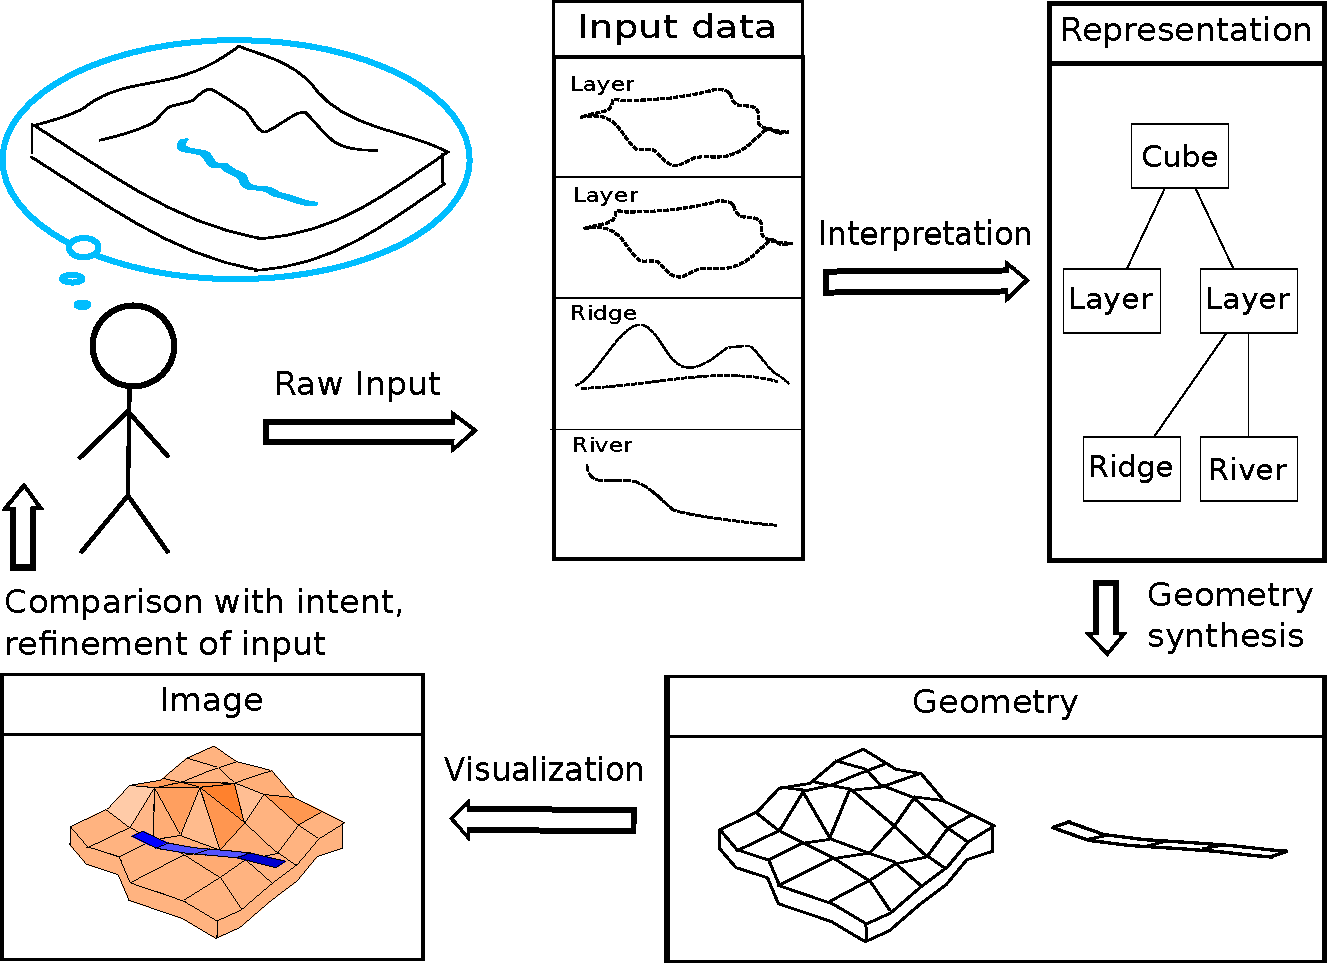
\includegraphics[width=\linewidth]{thesis/overviewConcept.pdf}
 \caption{Conceptual overview: The user has an idea in his head of what he wants to model. He indicates what he want to create to the program through various input methods. The program interprets the input, and for each feature creates a representation of it in the scene tree. The representation is then used to create new geometry and alter the shape of existing geometry. Once the geometry is ready, it is used for visualizing the results back to the user. The user then compares what he sees with what he had in mind. He can then do further refinement of the model by either changing what he already drew, or adding new features by drawing on the geometry itself.}
 \label{fig:overviewConcept}
\end{figure}

The aim of the internal format is to capture the modelers intent as well as possible. It is the the meaning of the input that is interesting and stored for the representation, not the geometry or how it looks. As we will see, this enables a modelling aproach that let's him to go back and change earlier things in the model without having to redraw everything, since all the geometry can always be recomputed from the internal format.

\clearpage
\section{Features}
There are a few different features that can be combined to create a scene inside the cube. Thes are layers, rivers, ridges, valleys, deposits and sea level. They can all be seen in figure \ref{fig:basicScreenhot}. The layers are created by drawing on the cube, while rivers, ridges and valleys are created by drawing on the layers. The sea level is simply indicated by clicking on the cube at the correct height. It can also be changed by dragging while holding the mouse button. The deposits are created procedurally by selecting a river, and then indicating that a deposit is to be made. The deposit will be made at the intersection of the river and the sea level.


% notes for methodology
%\chapter{Methodology}
% - how the algorithms works
% \section{Sketch methods and interpretation}
% - intersection\\
% - points are gathered\\
% - remove noise\\
% - auto-complete
% \section{Representation}
% - lines\\
% - surfaces\\
% - rivers\\
% - mountains\\
% - etc.
% \section{Geometry synthesis}
% - layers\\
% - mountains\\
% - rivers\\
% - sediments??
% \section{Rendering}
% - surfaces\\
% - rivers and overlapping\\
% - mountains
\clearpage
\chapter{Methodology}
\label{sec:method}
To develop a set of procedures and find a good solution to a complicated problem, one will find one self in need of a plan for how to do research and to approach the work itself. We will therefore begin with \secref{subsec:work}, by taking a look at how work was planned and how it progressed, from problem to general idea through reasearch, then implementation and refinement, to the final solution. 

We then proceed to explain the general design, algorithms and data structures used throughout the solution in \secref{subsec:generaldesign}. We explore how they work together to enable the drawing of sketches from input to finished model at a conceptual level. This part is intended to give an overview of how the algorithms work.

Finishing off the methodology section, we then take a more in depth look at the specific features of the program in \secref{subsec:indepth}. Here we will focus both on how different decisions about design were made, and go more in depth of how the implementation of each of the features of the program work algorithmically. Simple pictures that illustrate how the parts work are also included here.

\section{Work process}
Let's now take a look at the research and development process from start to finish. We'll begin by seeing how the first idea was formed, how the initial research proceeded and then move on to the implementation itself. Finally we'll consider how collaboration with geologists and students helped the progression of the project.
\label{subsec:work}
\subsection{Inspiration and research}
As mentioned in the introducion, work started with the percieved need for a tool to rapidly create three dimentional sketches for geologic structures. Various existing geological illustrations were investigated and there were some discussions about what would be the goal. At the beginning however, there was not a clear idea of to approach it or how this would be achieved. Research therefore started by reading some geologic papers and books, both to get an idea of what kinds of sketches was needed, what was to actually be sketched and to get a litte bit of an overview of what geology is.

This initial research turned out to be helpful. A large portion of the sketches encountered in litterature were drawn inside a cube shaped cutout. The cross section of the geologic structure along a primitive and easy to understand object like a cube, gives the viewer a good way of understanding how the different structures relate to each other. This was how the idea of the sketch cube, which is the starting point of the approach presented in this thesis, began.

Thus a vague idea of where to begin had been found. However, more details and strategies were needed to make the decision to proceed with that approach. Therefore a new research phase began, were techniques dealing specifically with sketch based input, procedural modeling, terrain modeling, geological modeling etc. were researched. A couple of example sketches that were found in geological papers, were used as a goal for what was to be possible in the program (see figure \ref{fig:initial1}). A set of different geological phenomena could be seen in these examples. Further research of modeling techniques gave some possible ways to do the input of such features, allthough the specific way to apply them to the cube methaphor was still unclear. Indeed, the way the cube and layers would be realized was not yet even clear. Nevertheless, an idea of how the finished solution could look and function from a users perspective was forming.

Hand drawn illustrations and an explaining text were made of how the finished solution was imagined to work, and put in a project description document. Figure \ref{fig:riverDesription} is an example illustration from that document showing how drawing of river structures was planned to work. The complete document can be found in the appendices. This was the basis for the implementation work at the beginning of the project. Of course a lot of further research and clarification of ideas was still needed, but since the general approach had been decided, the only thing remaining before implementation work could begin was to decide on technology. Such decicions  and the rest of research that was needed became guided by the implementation work itself, instead of the other way around. 

\begin{figure}
 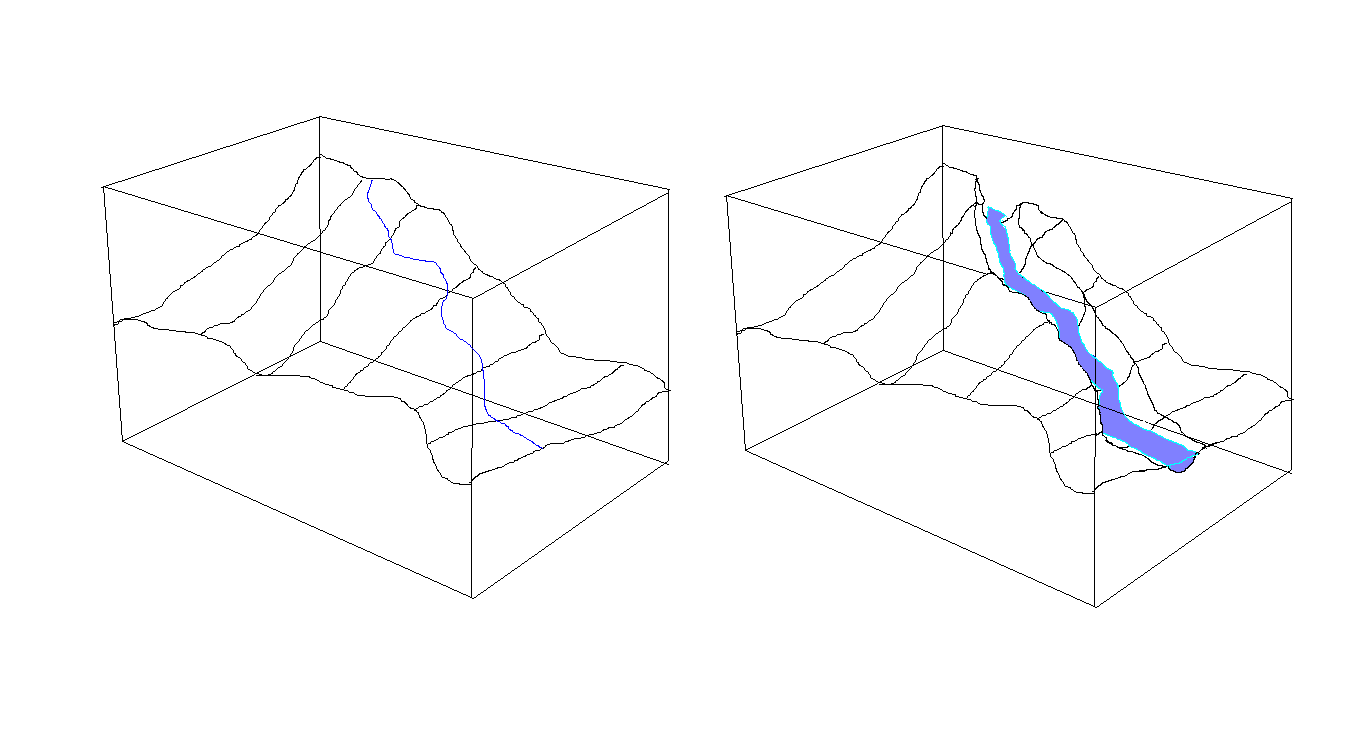
\includegraphics[width=\linewidth]{thesis/river.png}
 \caption{Illustration of how the drawing on rivers were planned to work at the beginning of the project, before implementation started. First, drawing a line on a surface where the rivers should go. Then, a river is created by an algorith in the program}
 \label{fig:riverDesription}
\end{figure}


\subsection{Collaboration}
After having created a version of the program that could be used as a prototype for demonstration, some outside collaborators from the department of geology were contacted. The rest of research and development was guided by the collaboration with them. 

The basic idea of the solution was shown to a professor of geology. He showed great interest and believed this could be good approach for illustrations in geologyband he had a few suggestions for improvements (see appendices for notes from the meeting). The main takeaway from this meating was that the focus on the ability of creating nice looking sketches in a quick fashion was the most important. There were also some other ideas and features suggested for further development. To help assess the development and suggest more improvements in the future, he gave the contact details of one of his students, Marie Songve.

%%%%%%    insert figure of sketch by marie, refer to it below

Marie helped develop some paper sketches that would be the main focus of development( see sketch in figure ILLUSTRATE ) from that point on. She also helped assess and guide the development through the rest of the implementation phase. In addition to giving concrete advice on the geologic features of the program, observing the usage helped identify the biggest user interface problems. After implementation Marie also helped in assessing the success of the project by giving her impressions and trying out the program by creating several sketches on her own. The results of this can be found in \secref{sec:results}. The collaboration with geologists was very helpful in guiding development direction and in taking choices during the implementation.

\subsection{Implementation work}

In this part the progression of work will be explained without going into much detail about the specific solutions created. The Only details included are those that are relevant for understading the most important choices which are discussed here and which are not explained earlier. For more details about the specific solutions, have a look at \secref{subsec:indepth}.

Implementation work was started by creating the cube and a camera system that would allow rotating around and zooming in and out of the cube. This was achieved relatively quickly. Intersection tests and input on the cube was the next step. At first this was achieved by simply looping through all the triangles and storing each intersection point in a list, and then drawing lines between the points that were drawn. However, the next step was the real challenge, which had not really been considered in depth until now. That challenge was how in the world to create a sensible layer from lines drawn on the faces of the cube. Different approaches were tried, and the details of how that turned out can be found in \secref{subsec:layers} further back. This ended up taking a lot more time that was initially expected. However, in order to focus on the solution, one has to know the problem, so all the work that might seem like a waste was actually needed in order to realize that there was a problem and therefore what 
kind of solution to look for.

Once a solution to the layer problem was found, there was of course a lot of other features needed to create a program that could be used for making useful sketches. Meetings with Marie helped focus the direction and prioritazation of their implementation. All the different features that were planned in order to reproduce the initial pen and paper sketch, were going to be implemented one after the other. Very often introduction of new capabilities meant going back and modifying existing code. In addition there were the non-geologic features of the program to think about, like undo functionality, save and load possibilities etc. These also had to work togheter with the other features in a way that would not upset any of the other features. As new features were added, it sometimes seemed as if the complexity was growing exponentially. It quickly became a problem keeping the different features working together in a smooth and predictable way. The program code was therefore changed many times to try and abstract 
the complexity to make the implementation of new features as easy as possible.

It was while realizing the complexity of the initial approaches that an idea of a parametric and ordered hierachical structure was introduced. In the start, everything was based on three dimentional coordinates, which made it difficult to calculate the relationship between for example the points on a layer and a river on it. If the layer changed, what point on the new surface would correspond to the beginning of the river? The user would have to draw the river again, which was not a good solution for a rapid modeling tool. The idea was that parametric coordinates would restrict the placement of a feature to two dimensions on it's parents surface. Thus, a new point in three dimentions could be calculated based on the parents position and geometry. The inspiration for this approach came from the paper by Schmidt et al. \cite{CGF:CGF1129}. This would ease the recalculation of coordinates once something changed. The ordered structure meant that each feature would only have to deal with immediate parent and 
children, and the order in which they had been drawn would be the guiding way to solve conflicts that might arise. The thought behind this was that the user would be thinking of the structures in a hierachical way already, and after familiarizing himself with the program would know in what order features need to be drawn to create the desired effect. After all, it does not make sense to have a river without first having a surface on which it flows.

The parametric and hierachical solution could now be used for many problems. For example, how does one specify the height of a ridge and how does this height change if the layer changes, and how and where does it affect the underlying parent? The simple solution was making the ridge baseline a parametric coordinate on the layer, and for each point along the baseline, there was associated a height value, which could then be used to compute the actual resulting top point of the ridge by first finding the position of the baseline point on the surface, and then adding the height. How to do the actual morphing of the underlying surface to create the ridge also became a lot easier, since the lookup of surrounding points now was restricted to two dimentions and the baseline point was already known in this space.

There were of course a lot of other difficulties remaining to solve to reach the stage the program is in now. However, the rest of the development was more about smaller issues local to each problem, and will be covered in the relevant subsection in \ref{subsec:indepth}.  There were still complexity issues of course, about how to fit each feature into the general solution without interfering with what was already implemented. New ideas were developed as work progressed, and others discarded along the way, mainly for lack of time. Going into all those details would mean we could write several books, but the details about solutions that have been implemented, and the problems and their solutions that are relevant to understanding choices will be included in the next two sections.

\section{General design solutions}
\label{subsec:generaldesign}
In this section we will explore the general concepts that all of or most of the features have in common. After follows a more in depth explanation of each specific feature.

There are three abstract steps from user to the visual image. These the input interpretation, the geometry synthesis and visualization as explained in \ref{sec:concept}. After input has been gathered and the users intent understood, the interpretation algorithms creates a structure that hopefully captures what was intended. The third step is then to create a geometric representation of this structure for use in the visualization step. This is often the most computationally heavy process. The visual feeback of the produced image to the user will then enable him to refine his input, should it be needed, such that the image better represents what he originally had in mind. 

From the users perspective there is a certain structure he wants to model. In his head he has an abstract notion of each of the parts that are needed and a notion of the image he wants to produce. The user knows how to input parameters that the program will interpret in a certain way to create the structures he intends. Thus the first step of the program is to interpret the users input.

\subsection{Sketch input and interpretation}
The initial state for input is the empty cube. At this stage the input consists of the user rotating and drawing on the cube to create layers. Rotating is, as mentioned earlier, done by dragging the mouse while holding a button. In code it is trivial to achieve by just rotating the camera a certain amount according to how far the mouse was dragged. The camera object itself is implemented as a class that has a position, a point of rotation and a field of view. I also methods for moving it around, rotating it and for creating a transformation matrix for the opengl viewport. The camera is used in the input stage in order to know the direction and angles of the viewport, so that the input from the user can be transformed to the correct coordinate sytem from the two dimentional screen space to the three dimentional space of the representation.

 To achieve the correct capture of the users input it is first neccessary to find the correlation of where the user draws on screen and where this corresponds to on the cube. The drawing of curves is acheved in the same manner for all objects in the scene. For this purpose one must know the camera position, camera direction, viewing angle and viewport size. When there is a mouse position somewhere on the screen it is then realatively easy to compute a direction vector from the cameras position and into the scene that will point at the position on the cube that lies under the mouse pointer. When this vector is known, finding the exact point on the cube is a matter of intersection between a ray and a triangle. For most objects there is a structure that contains all the triangles it consists of. Each of the vertices of the triangles are stored together with parametric coordinates that uniqely represents the point on the two-dimentional surface of the object.

While drawing on a surface the three-dimentional intersection points in the scenery space is stored in a list in order to immediately visualize it to give the user feedback. The two-dimentional parametric coordinates are stored in a seperate list for later use.

When drawing on a screen you are limited to the resolution of the screen. This means that the input points that are gathered will also be limited to this resolution However, because the actual surface where you are interested in drawing exists in a point in space farther away and not on screen, moving from one pixel to the next, means you will move a much greater distance on that surface than on screen, creating jagginess. Also, depending on the angle and distance of the camera, the jagginess you get will be uneven. For this reason we need do smooth the input points that have been gathered. 

The smoothing is done by regarding the n points of the  input as the control points of a n-dimentional bezier curve. This is done in the two dimentional parametric space. The rationale for doing it this way, is that the points gathered are usually not on the line where you wanted to draw, but will lie on either side of the actual line desired. The bezier curve will aproximate the control points, but will lie somewhere between them as illustrated in figure \ref{fig:bezierSmooth}. Thus, since most of the points lie on either side of the actual line, what we want is for the actual line drawn to lie somewhere between. If enough control points were gatehered from the input, this is what we get.

An alternative considered for the input, was to use a hermite spline such as the Catmull-Rom spline. However, this approach did not give nice results, as the control points were too noisy, and since the hermite spline interpolates all the control points, this gave too many unwanted artifacts as the line would have to wiggle around to achieve that. Since the control points do not lie on the actual desired line anyway, but rather lie on either side most of the time, interpolating the points is not what is desired anyway.

\begin{figure}
 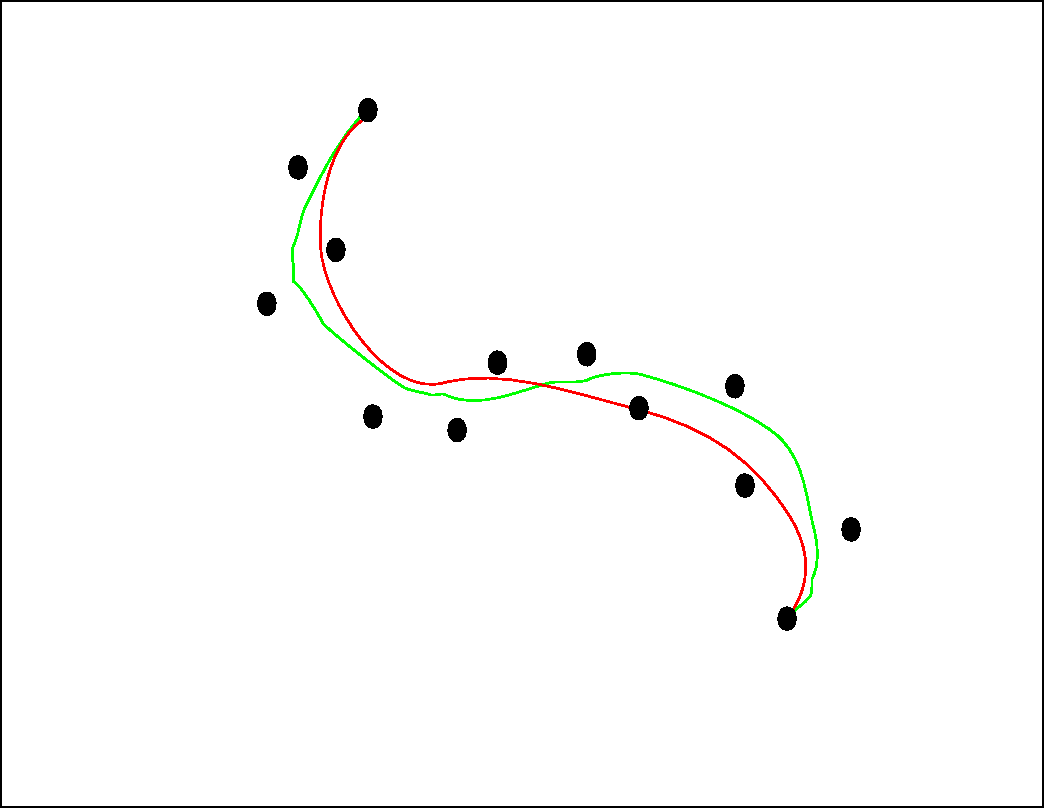
\includegraphics[width=\linewidth]{thesis/bezierSmooth.pdf}
 \caption{The green line indicates the mouse movement and how the user would expect the line to appear. the black dots are the actual points gethered at the surface from the intersection tests. When using these points as input for a bezier curve, we end up with the red line.}
 \label{fig:bezierSmooth}
\end{figure}


A similar but more advanced approach can be found in the stroke capture section of Cherlin, 2005 ~\cite{Cherlin:2005:SMF:1090122.1090145}, and that is where I got the idea for using bezier curves from. However, I found the current procedure to give adequate results and did not spend more time on improving the input interpretation.

It is also possible to oversketch the lines that are already drawn. The oversketching principle was mentioned in \ref{sec:star}. The are many ways to implement oversketching, and each use case might be different. The oversketching methods in the application are different according to the context and what the current task is. When drawing the layers, the oversketched lines are simply replaced for the section of the original line that is closest to the new line. While changing a ridge height, the new line replaces the points below, and while changing the sides of rivers and valleys, the procedure is similar to the layers, only incorporated into the original line with a function that smooths the transition more. The details of each of these will be explained better in \secref{subsec:indepth} under the relevant feature explanation.

Once the input has been interpreted, the new data (or changed data) will be stored in memory in a representation specific to the kind of feature the user has indicated he wants.

\subsection{Representation}
The different features that can be drawn are, as mentioned earlier, represented in an internal format before creating the structure that can be visualized. Relevant parts of this representation is also visualized to the user in a way that he can uderstand it. This makes it easier to make changes, and reason about what can be changed and what effects that will have on the final result.

The curves are as mentioned stored as a list of points. On a higher level of abstraction, most of the features that can be drawn are built by using such curves in different combinations and different interpretations. In many cases the curves are augmented by some additional information, such as the height of ridges. In one instance, the deposits, the representation does not include lines at all but their shape is rather defined by a procedural method.

All the features relate to each other in a child-parent relationship creating a tree structure. The cube is the top node in this tree. All layers are children of the cube. All the other features are then the children of a layer, as can bee seen in figure \ref{fig:tree}. This structure toghether with the parametric representation is useful to enable incremental refinement of features, meaning that any part of the whole structure can be modified at an time, withouth having to redraw every part that relates to that change. When a node changes, it knows whether it needs to tell the parent and a parent knows whether it needs to trigger some recalculation in a child. Such notifications are however only sent along and used for telling the geometry synthesis to do neccessary recalculations, since the parametric representation itself does not actually need to change. Schmidt and Singh 2008 \cite{CGF:CGF1129} was an inspiration for this parametric and hierachical way to represent the sketches.

\begin{figure}
 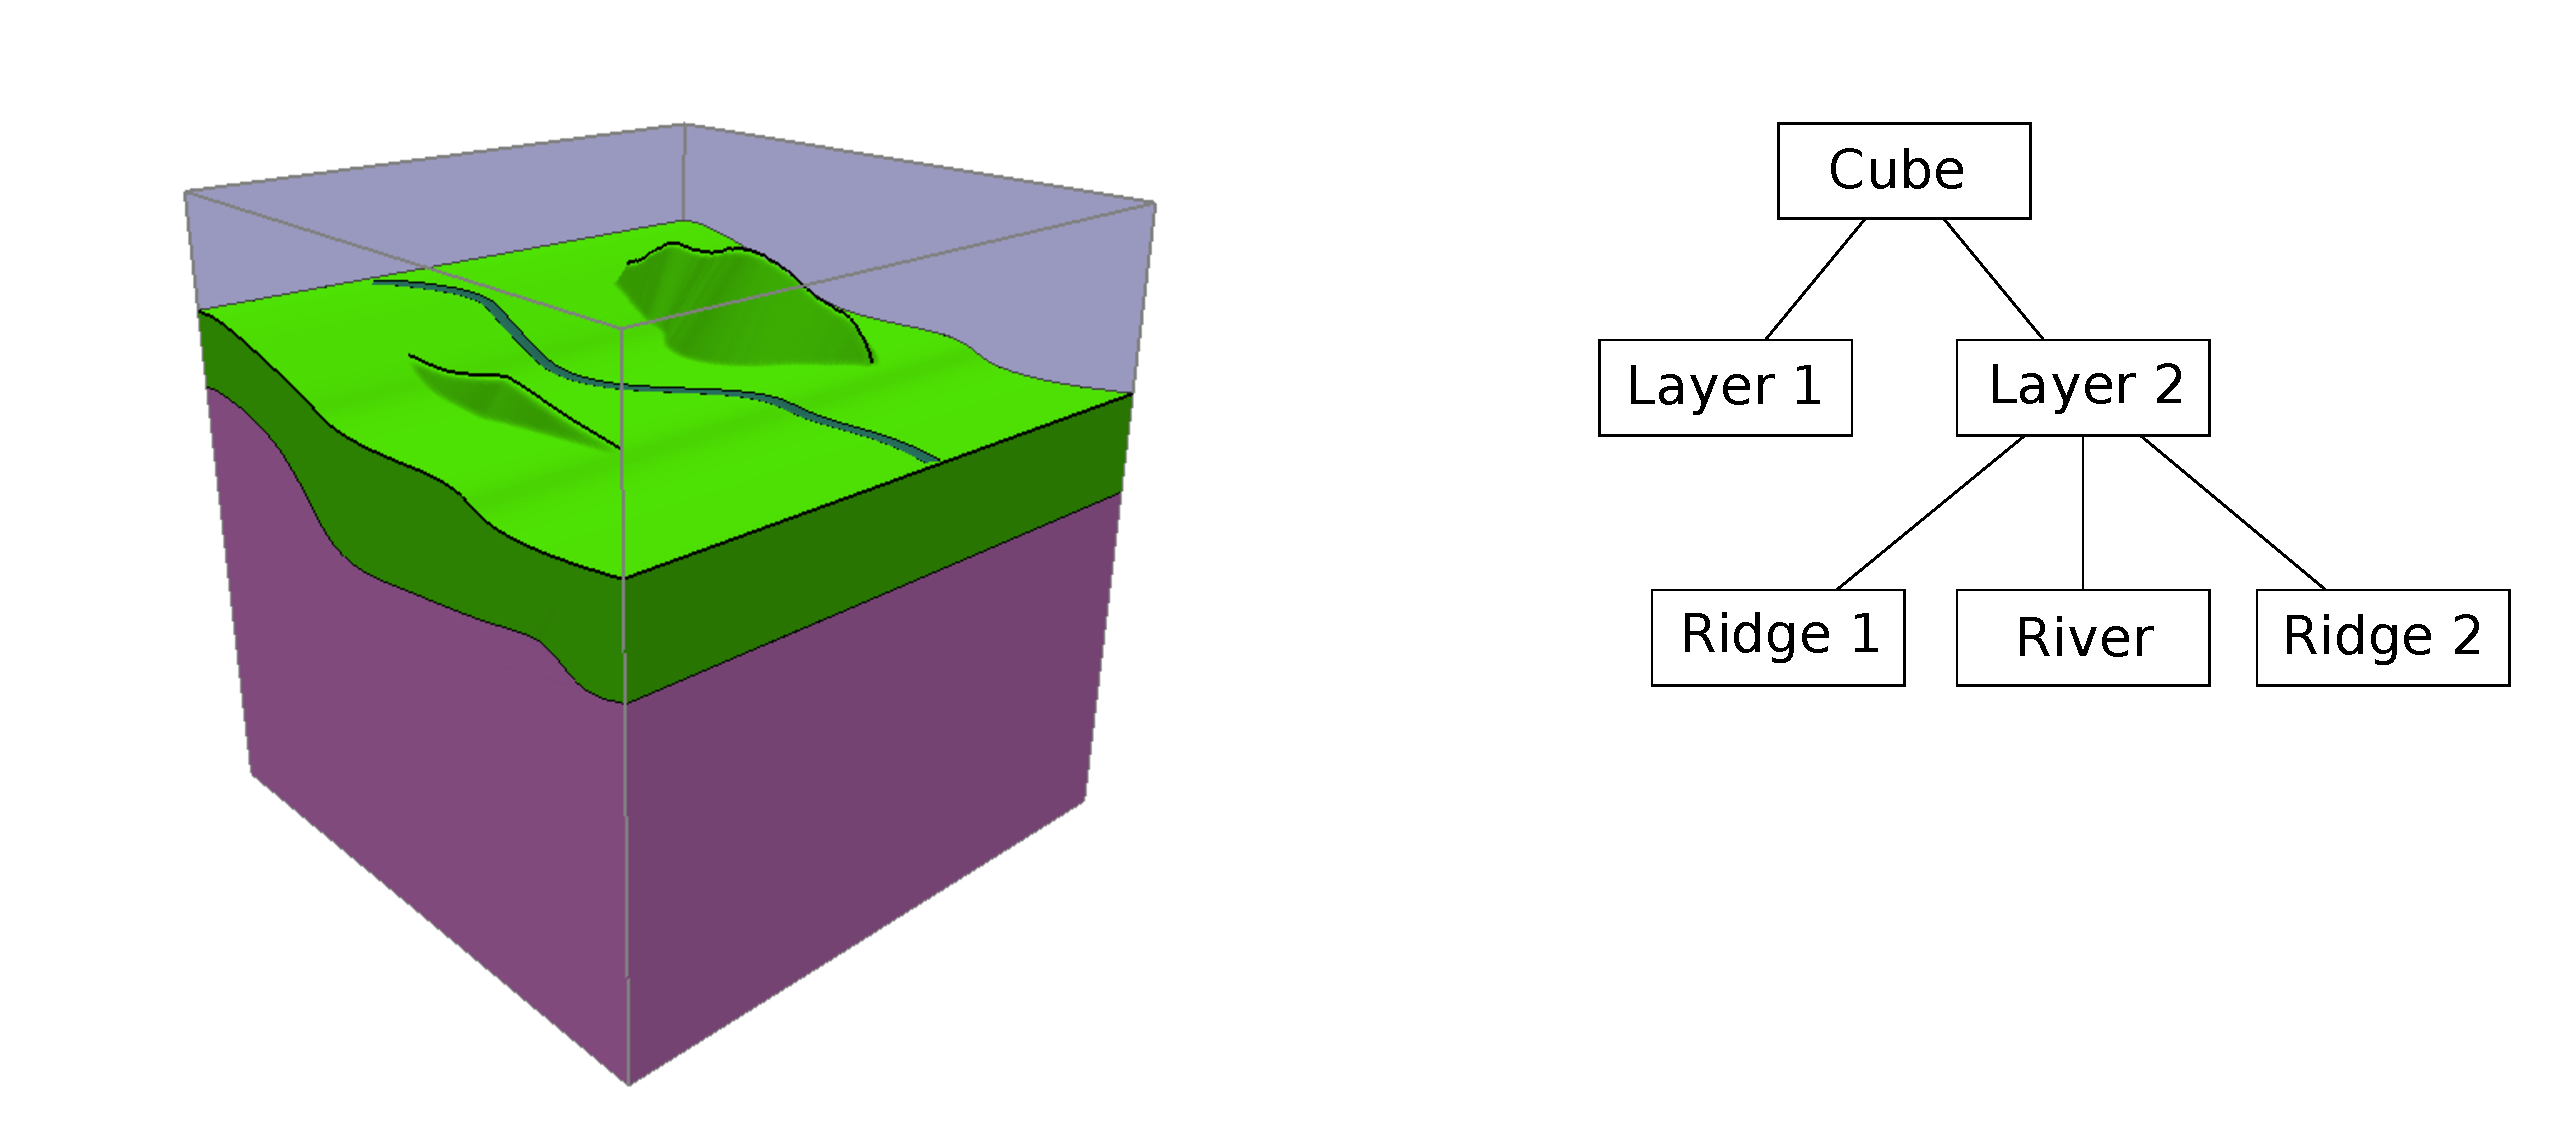
\includegraphics[width=\linewidth]{thesis/tree.pdf}
 \caption{The scene is represented by a tree of nodes, where each features gemoetry and position is calculated according to the relationship with it's parent. On the left we see a scene where there are two layers drawn. On one of the layers there are two ridges and a river drawn. This results in a tree structure like the one on the right}
 \label{fig:tree}
\end{figure}


\subsection{Geometry synthesis}
Before a certain scene configuration is visualized, a geometry is created. For each type of feature in the scene, there is a corresponding algorithm for creating the relevant geometry. When the layers geometry is being constructed, it needs to take into account the children. This is because some of them can actually change the surface of the layer. Each node in the scene will keep it's geometry so it does not need to be generated over and over. When it needs to update, it will be notified, and trigger it's relevant algorithm for generating gemoetry.

\subsection{Visualization}
The visualization is achieved by a geometry object associated with each feature. It has an array with vertices and associated normals. This class is also responsible for intersection testing, and thus has the associated parametric coordinate of each vertex to be able to interpolate this value from the three vertices of a triangle where an intersection has been found. Simple opengl functions are used for drawing the triangles. To achieve transparency, care is taken to draw the transparent objects last. The shape object also has a list of points that it uses to draw strips of lines if present. This is used to visualize all outlines of objects and curves. There is also a three color vectors for a shape to enable material for the different gemoetries.

\section{Specific solutions}
\label{subsec:indepth}

Here we begin by taking a look at the choice of technology like programming language and libraries. Then we continue on to have a look at each specific feature and how each of them were realized in the context of the design explained earlier. Algorithms of special relevance will also be given in pseudocode, explained and illustrated. All of the features will be explained by referring back to the previously explained steps of input, representation and geomtry synthesis. Any alternative approaches considered and rationales for the choice made will also be discussed.

\subsection{Technology}
The choice of technology to base the work on was made by a bit of trial and error. Different scene graphs in c++ and Java were tested to see what would work the best. In the end it was decided that the project would be based on c++ as programming language with qt for user interface and opengl for graphics. Custom visualization and scene graph code would be created, as some specific things would be needed that might not fit nicely into a premade solution. 

Qt was chosen as the user interface library because of previous experience. In addition to having a good set of user interface classes it also has a lot of helpfull classes with things like collections and event handling that make the process of programming in c++ pleasant.

Some tests were initially conducted in java by porting the code from c++ as it was made. Allthough the java runtime itself is theoretically fast enough, naívely using it's methods of abstraction slows down data access a lot. This forces you to write complicated and unreadable code that defeats one of the main purposes of using jave in the first place. The abstractions in c++ can be a bit more complicated to use than in standard Java, but also allow much faster data access and better control over memory allocation. The main problem here was that Java would constantly allocate objects on the heap even though they would only be needed temporarily. The Java compiler does have optimizations that removes such allocations where possible, but a lot of times it cannot know what the life expectancy of an object is. This was possible to overcome by writing specially designed code to make it possible for the compiler to see where a temporary object is not being reused and by passing primitive types in stead of pointers 
to objects in many places. Another problem is that arrays are restricted to contain primitive types or pointers. Thus an array of objects cannot be allocated such that it's objects lie in contigous memory, and this slows down access a lot. This was also possible to overcome by making arrays of primitive types in stead of objects. Bith these approaches put together made the code run comparably fast to the c++ code, but also almost as hard to understand and modify as assembly language, and therefore I decided against continuing this approach. It would probably have been possible to solve all such problems with Java by relying on doing all heavy calculations on the GPU by using opengl shading language or a similar GPU programming language. This was decided against for lack experience with GPU programming and a lack of time for learning and experimenting with development tools designed for such programming. None of the algoritms explained utilize this possibility, allthough that would probably increase the 
running speed noticeably.

\subsection{Cube}
There is no input to change the parameters of the cube. The cube itself is represented by the size of its three dimensions. That is, height, width, and depth. It the outset it was the intention to be able to change the size of the cube in these three dimensions, but there was not enough time to get to this feature. The gemoetry of the cube is constructed by creating and positioning six square faces of correct size and the correct orientation. Each of the faces are also in turn contructed by two triangles and outlined by a line strip. When visualizing the cube geometry, only the triangle of the back faces are rendered, but all lines are shown. This effect is achieved by backface culling, makes the cube look transparent, and avoids occlusion of the geometry inside. The cube can also be made invisible like other objects, which can be useful for making screenshots where the cube is not neccessary.

\subsection{Layers}
Layers can be created fast and easy. In figure \ref{fig:layerCreate} we see how a layer is made by first drawing the four curves on the side of the cube, and then letting the program create the layer surface. A surface like this can be created in about 30 seconds.

The layer can also be edited. When editing, the old curves are shown with a red stippled line while the new line that is the result of oversketching is drawn with a black solid line, as can be seen in figure \ref{fig:layerEdit}. Once done editing the program will compute new geometry for the layer based on the new curves.

New layers may be added on top of existing layers as seen in figure \ref{fig:layerNew}. If the layers intersect, only the part that is above the previously created layers will be visible. If the new layer intersects with previously drawn layers, only the part that is above will be drawn, as seen in figure \ref{fig:layerIntersect}

\begin{figure}
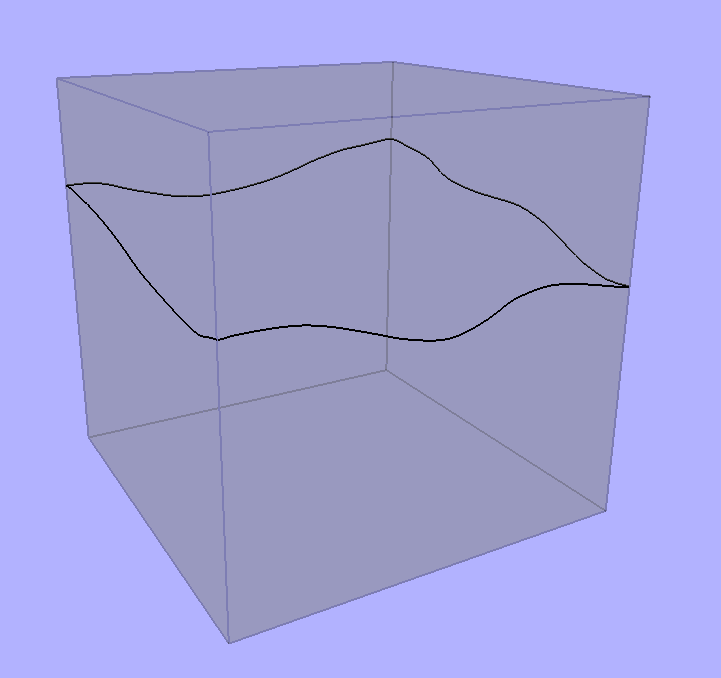
\includegraphics[width=.5\linewidth]{thesis/results/simpleLayerDraw.png}
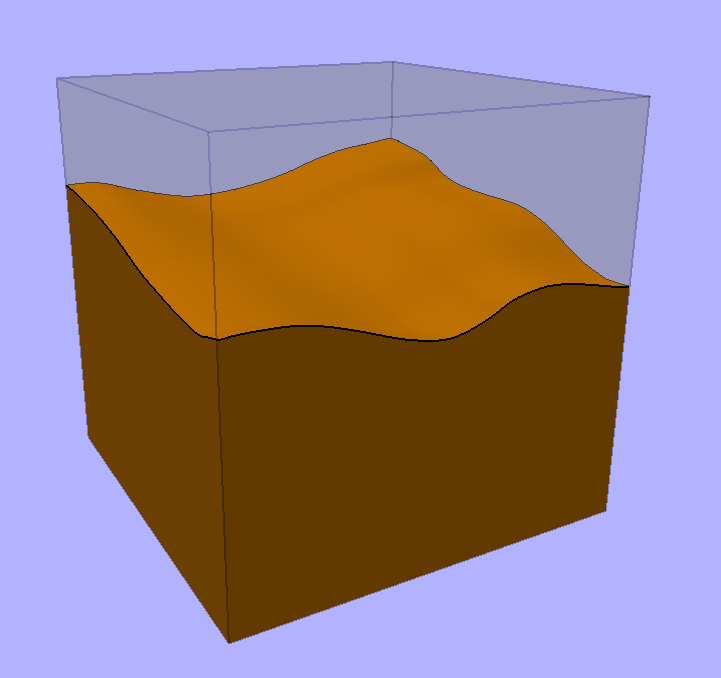
\includegraphics[width=.5\linewidth]{thesis/results/simpleLayerCreate.png}
 \caption{The layer is represented by the four curves the user draws, plus the lower line that represents the top of all previously drawn lines. The layer geometry is generated between these two lines.}
 \label{fig:layerCreate}
\end{figure}

\begin{figure}
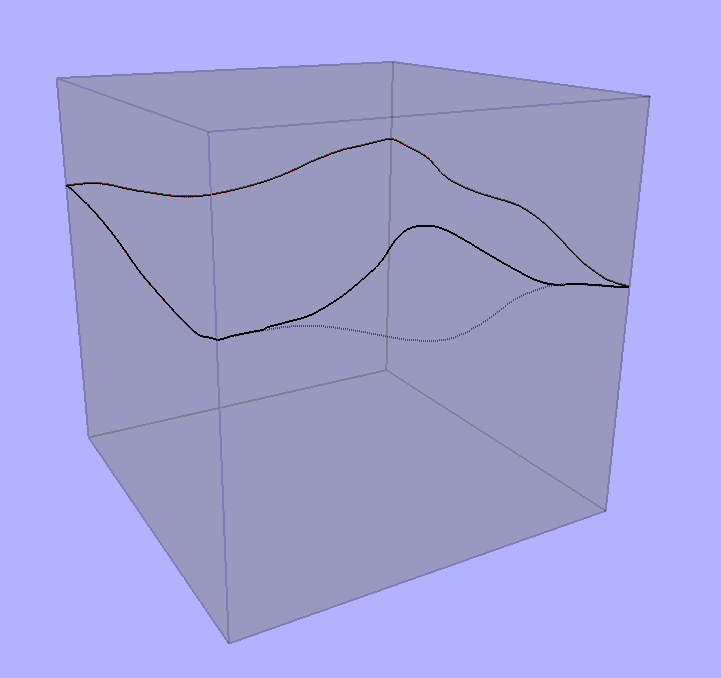
\includegraphics[width=.5\linewidth]{thesis/results/simpleLayerEdit.png}
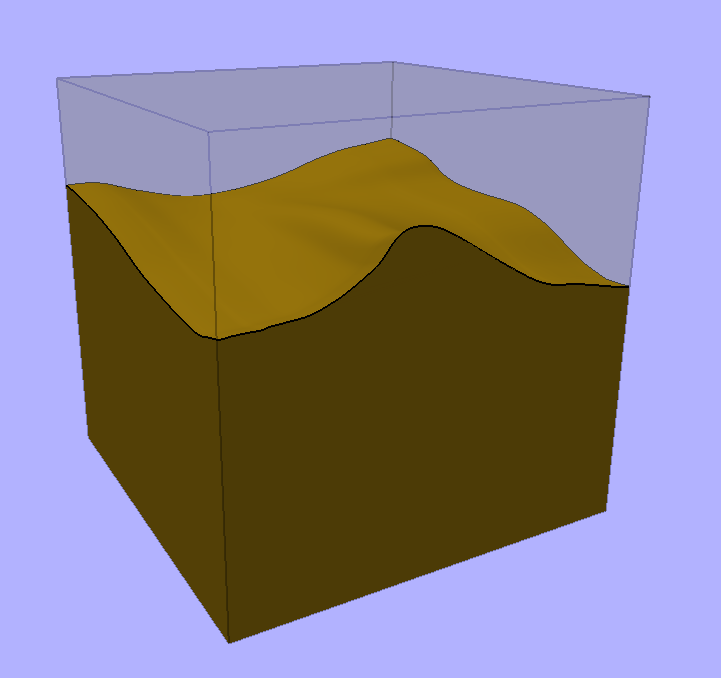
\includegraphics[width=.5\linewidth]{thesis/results/simpleLayerEdited.png}
 \caption{Layers can be edited. The left hand picture shows the old curves in red, and the new curves in black. On the right we see the resulting layer after editing.}
 \label{fig:layerEdit}
\end{figure}

\begin{figure}
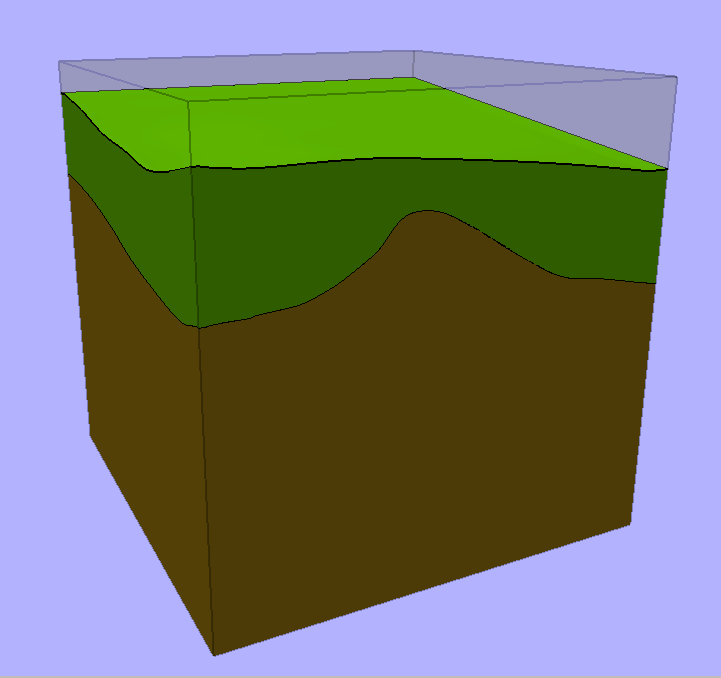
\includegraphics[width=.5\linewidth]{thesis/results/simpleLayerNew.png}
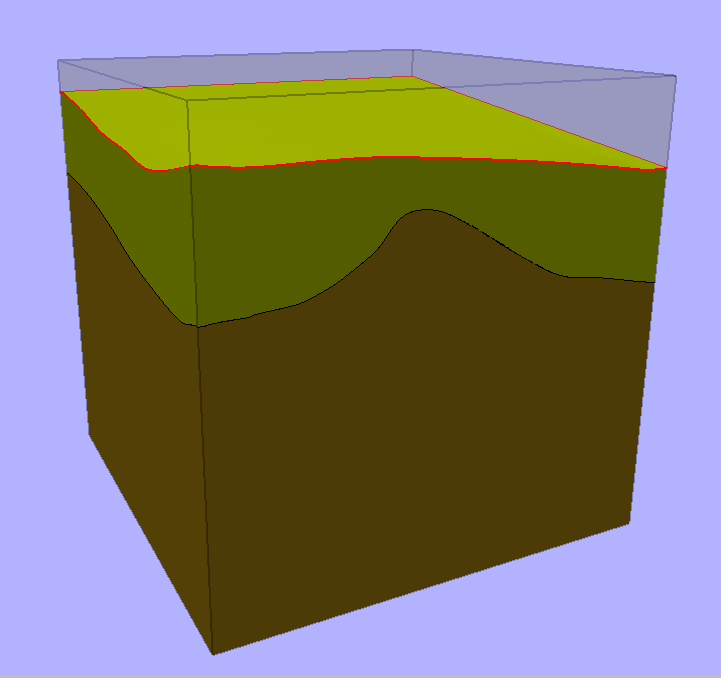
\includegraphics[width=.5\linewidth]{thesis/results/simpleLayerNewMarked.png}
 \caption{It is possible to create multiple layers as can be seen here. When one has multiple layers, it is also possible to select one of the layers by right clicking it, as seen on the right. When a layer is selected, it is highlighted by a slightly brighter color, and it's outline is drawn in red.}
 \label{fig:layerNew}
\end{figure}

\begin{figure}
 \centering
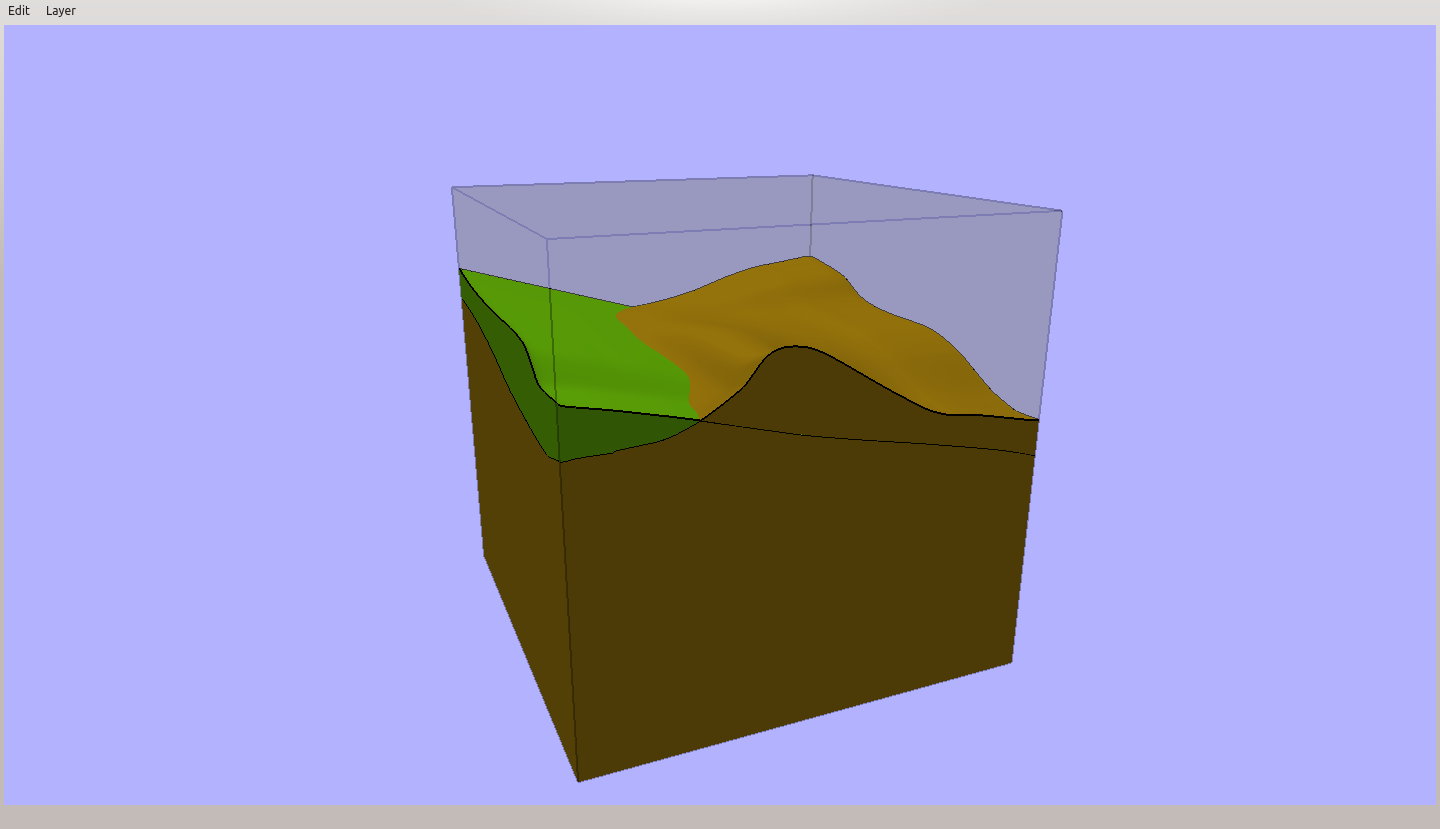
\includegraphics[trim = 90mm 7mm 80mm 30mm, clip,width=.5\linewidth]{thesis/results/simpleLayerIntersect.png}
 \caption{Layers might also intersect with each other. In that case what is above of the last drawn layer will be what is visible, while what is below is not part of the new layer.}
 \label{fig:layerIntersect}
\end{figure}

\label{subsec:layers}
At the onset of development, while the final solution was still only an idea, creating the layer wasn't really considered to be a challenge deserving all that much consideration. However, a considerable amount of time was spent on figuring this out. The very first thing done was to simply loop through all the points and draw triangle strips beginning with the first and last point, then second and second to last, and so on. This created some structure that could resemble a layer, but it was clear that it would not be usable for anything, and it was not very robust at all. The second approach was to do a simple interpolation of the points on the cube faces for each point, by going from left to right, back to front of the cube along the curves drawn on the cubes faces. Before this could be achieved, it was then clear that the four sides of the cubes needed to have separate structures and detection of which face was being drawn on. This was achived by creating a separate structure out of each side, and making a 
base class that would become the basis for the tree structure that eventually became an important part of the final solution. Thus, each face now kept track of it's own point as they were being drawn on.

The interpolation of a layer from these points did work to create a surface structure, and it was a robust solution. The problem was that it did not interpolate each point that had been drawn on the cube, and thus it was difficult to predict what you needed to draw in order to get the desired result (INSERT ILLUSTRATION). A solution where the user coud expect the layer surface to pass through the actual points he would draw was desired to achieve the goals of being a tool for rapid sketching that did not require advanced training. Another solution would therefore need to be found.

A lot of time was spent in order to find a satisfactory solution to this problem. Books on curves and surfaces were read for a while, but in the end the solution came from the geologic field itself. A technique that geologists use to model surfaces in sand was stubled accross. This old technique involves using two wooden profiles, and then slide a third profile across to create a surface. The technique is depicted in figure \ref{fig:wooden} and how it was adapted for the final solution is described later in \secref{subsec:indepth}. Another technique was also developed concurrently with that approach, inspired by Inverse Distance Weighing interpolation, but only using the four perpendicular points like in the other approach and weighting them. The points were weighted by the function $1/distance$ if distance were more than 0. If distance was 0, only that point was used. This yielded similar results, but results was a bit more unpredictable when making a complex surface. Also, the irregular grid tended to get distorted according to how close to the edges a point on the grid was. This created further problems with the parametric space later. For these reasons that approach was not included in the final solution.

Input for layers are drawn on the cube faces. On faces where the user draws, there is an auto-complete function while on the left, right and oppsite side there is a suggestion function. The simple auto-complete will automatically complete a line you draw by extending it towards the left and right side of the current face. 

\begin{figure}
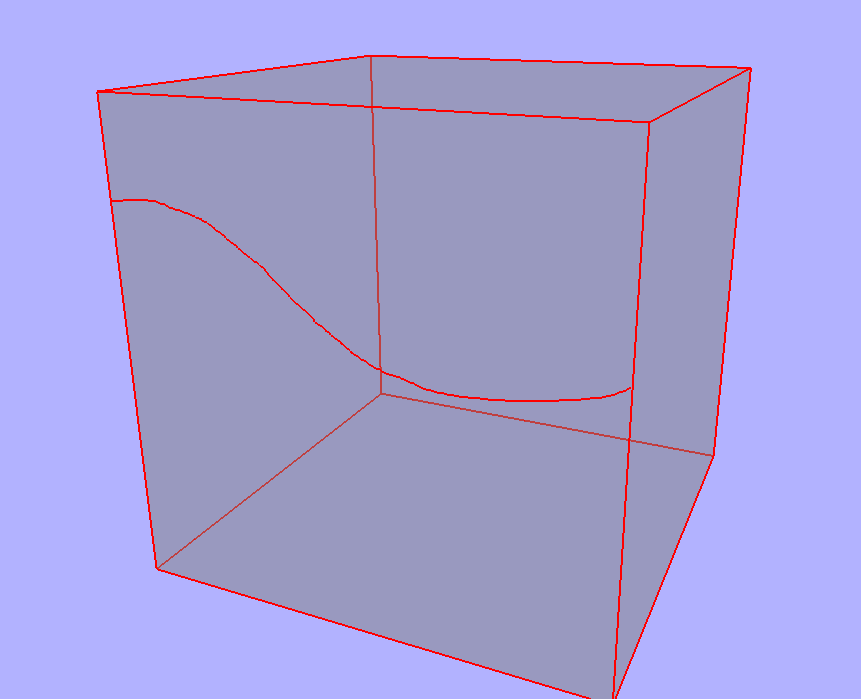
\includegraphics[width=.5\linewidth]{thesis/suggestion1.png}
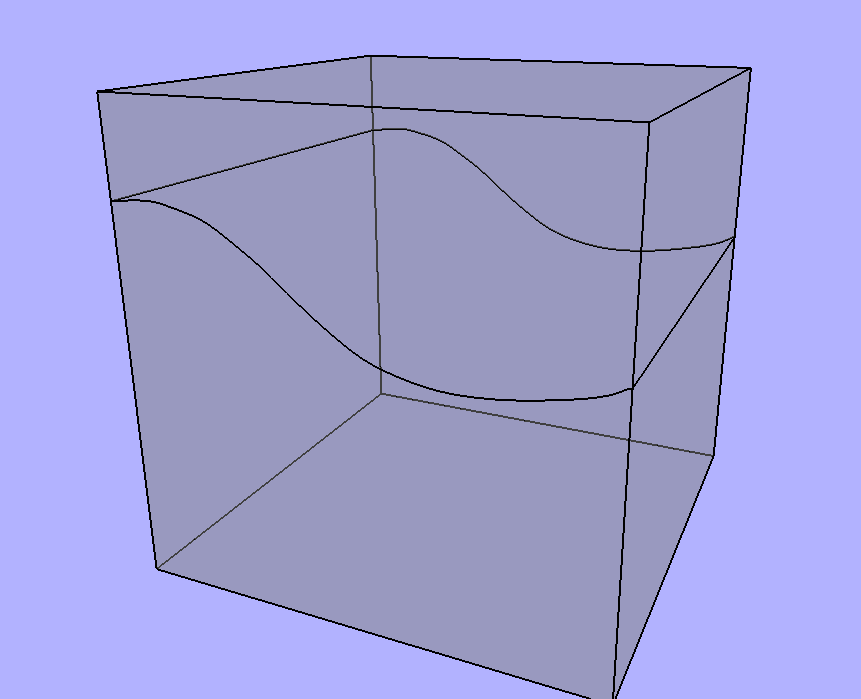
\includegraphics[width=.5\linewidth]{thesis/suggestion2.png}
 \caption{When the user draws the first curve on a face of the cube, it is replicated on the opposite side, and then lines extended on both left and right hand sides.}
 \label{fig:suggest}
\end{figure}


The suggestion does different things according to the state of the other faces. If there has been no user input on the opposite side of the cube, it will automatically mirror that input to that opposite side of the cube from where he is drawing, and then extends lines between the first and last point of the curve on the current face to the first and last point of the curve on the opposite face. (see figure \ref{fig:suggest}) These straight lines will then of course end up on the faces to the left and to the right of the face the user is currently is drawing. When further changes to this initial suggestion are made, what will happen depends on which sided have been draw on directly by the user already. ( see figure \ref{fig:layerModify} ) If the opposite face has already been drawn on by the user, it will not be changed. If the left and right side has been draw on, they will be modified so that the first point aligns with the last point of the left hand face, and the last point aligns with the right hand face.
 This is done by imagining a line from the first and last actual points of the curve, and then replicating the distance in height of each point on a new imagined line in the desired position ( from the new point at the beginning or end of the recently modified curve to the opposite side ). Otherwize there will simply be drawn a straight line fitting the same 
constraints. This assures that the lines on all the faces are always connected at the edges of the cube such that they are always ready to create a layer from.

\begin{figure}
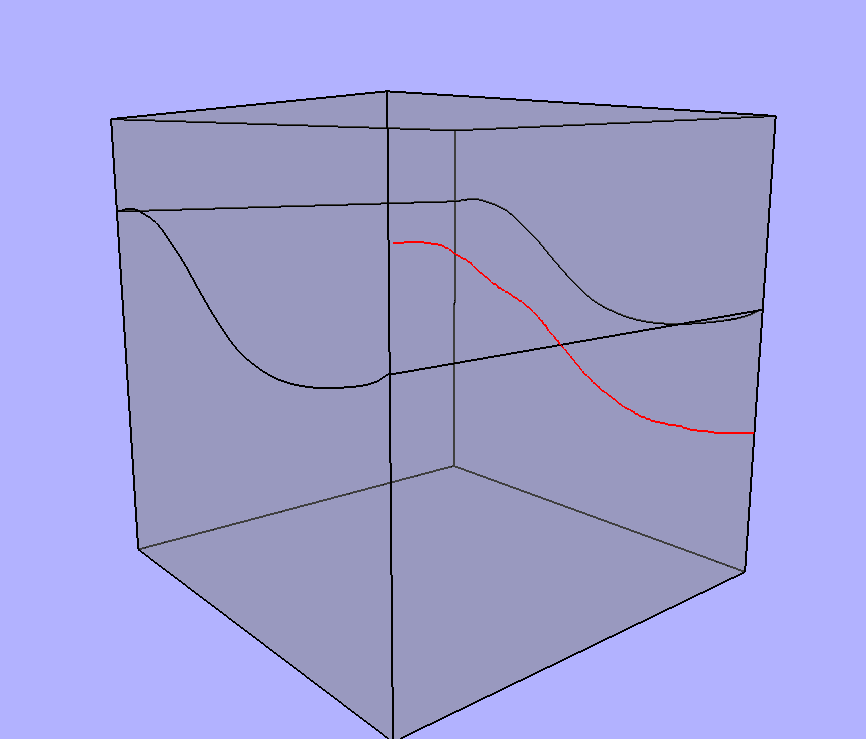
\includegraphics[width=.5\linewidth]{thesis/modification1.png}
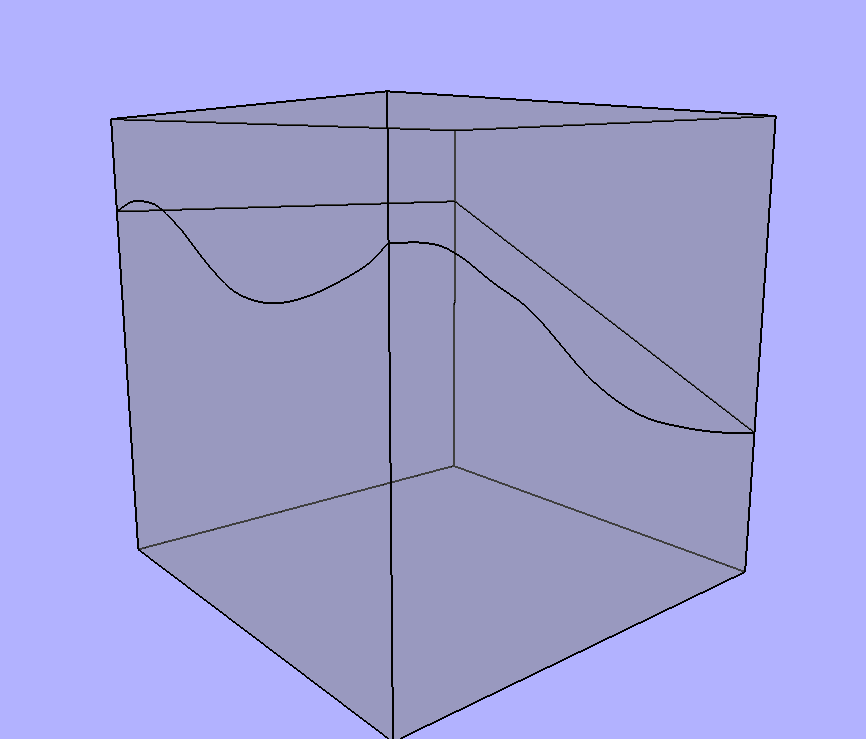
\includegraphics[width=.5\linewidth]{thesis/modification2.png}
 \caption{When the user modifies a preexisting face of the cube different things can happen. On left hand side we see that the curve that was drawn earlier is modified to line up with the new endpoint. On the right hand side, which was a generated line, we simply generate a new line like earlier. On the opposite side nothing changes.}
 \label{fig:layerModify}
\end{figure}

A Layer is represented using 8 curves. First, the four curves from user input on the cube is used to create a surface representing the top of the layer. Then, for each of the sides, the users input on this side and a precomputed line that represents the bottom of the layer (that is, where it meets the surfaces below) are used to create a surface for the side of the layer. This bottom curve is thus actually imlicitly given by the previous layers that already exist, and thus it is actually all previous layers that are part of the layers representation and the bottom curve is not really needed to be able to recompute the layers geometry. It is kept temporarily though, in order to avoid unneccessary recomputing it. === FIGURE illustrating the representation of a layer ===

\begin{figure}
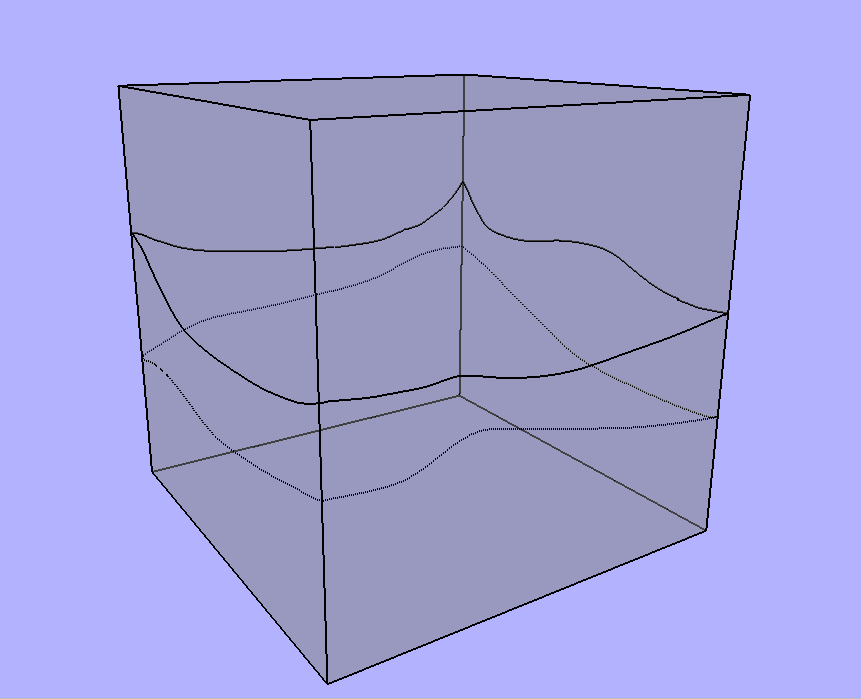
\includegraphics[width=.5\linewidth]{thesis/layerRepresentation1.png}
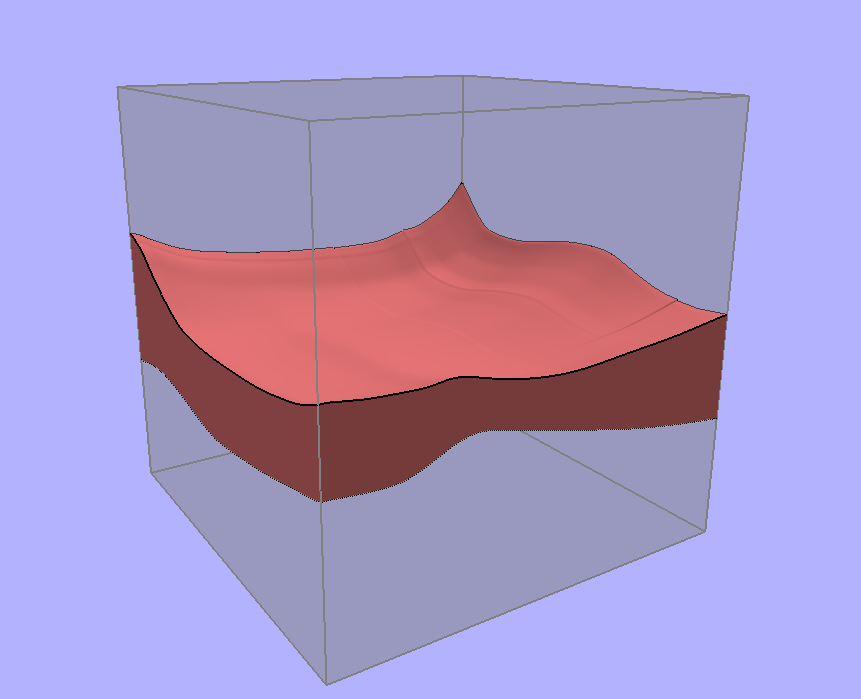
\includegraphics[width=.5\linewidth]{thesis/layerRepresentation2.png}
 \caption{The layer is represented by the four curves the user draws, plus the lower line that represents the top of all previously drawn lines. The layer geometry is generated between these two lines.}
 \label{fig:layerRep}
\end{figure}


Below I present an algorithm for creating a height field from these four curves. The inspiration for this algorithm comes from an old technique used in geologic modeling in sand. I read about this technique in the book Curves and Surfaces for CAGD, by Farin \cite{farin2001curves}. In this book it is simply used as an example of pre-computer surfaces, so it was somewhat of a concidence that I found this technique here. The idea is that you can model a suface in sand by carving two profiles on the left and right side of a wooden box. Then, by dragging a third free hand wooden profile along the two sides you modify the sand surface accordingly (see figure ~\ref{fig:wooden}). The algorithm I present here can be thought of as very similar, only it will allow you to create two versions of the free hand profile, between which the actual profile will be interpolated at each point as you drag it accross the sides.

\begin{figure}
 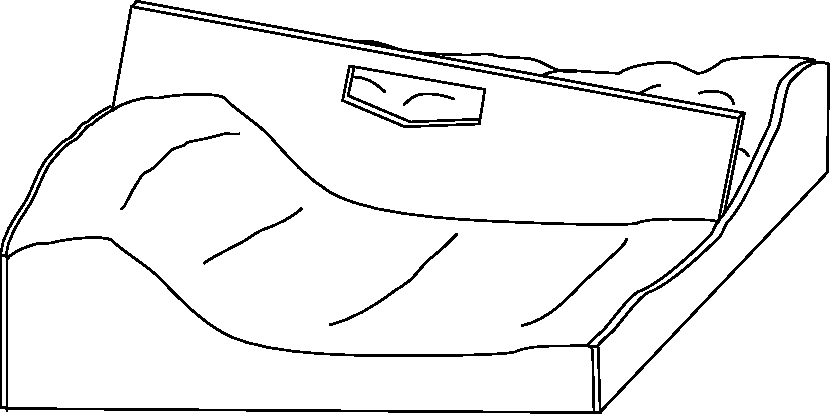
\includegraphics[width=\linewidth]{thesis/sandbox.pdf}
 \caption{Modeling a surface in sand, by dragging one free curved profile across two different fixed curved profiles on either side of a box filled with sand}
 \label{fig:wooden}
\end{figure}


Construction of the layer surface geometry is achieved by looping through the lenght of the curves drawn on the cube, from left to right for the front and back curves, and for each of these points, again looping through from the front to the back of the left and right curve. These points are of course stored as two dimentional parametric coordinates, but can easily be translated to three dimentional coordinates. If we then call the three dimentional points of the left, right, front and back curves Cl, Cr, Cf, and Cb respectively, and denote the point along them as Cl(x), Cr(x) and so on, where x is a value between 0.0 and 1.0, we get a grid of new points that represent the heights of the surface according to this algorithm:

\begin{algorithm}
\begin{algorithmic}
\ForAll{points in grid(i,j)}
  \State $left \gets Cl(1)*(1-j) + Cl(0)*j$
  \State $rigth \gets Cr(0)*(1-j) + Cr(1)*j$
  \State $start \gets left*(1-i) + right*i$
  \State $frontBack \gets Cf(i)*(1-j) + Cb*(1-j)*i$
  \State $leftRight \gets Cl(1-j)*(1-i) + Cr(i)*i$
  \State $difference \gets frontBack - start$
  \State $grid(i,j) \gets leftRight + difference$
\EndFor
\end{algorithmic}
\end{algorithm}

Explained in words, first interpolate the four corners of the cube according to the coordinates i and yielding a starting point for the surface. Then interpolate the front and back curve points Cf(i) and Cb(1-i) using the j coordinate and calculate the difference from the starting point. Then interpolate the left and right curve points Cl(j) and Cr(1-j) using the i coordinate. Add the previously calculated difference to this point, yielding the final point. The effect of this algorithm is analougous to the magically changing wooden profile explained earlier begin dragges across the left and right curves while the actual profile is the interpolated front and back curves. The effect of the algorithm is the same no matter if viewed as if dragging the front and back interpolated curves across the left and right curve or vice versa.

Another algorithm was implemented and tested. The idea there was simply to loop in a similar fashion, but directly interpolate the four points Cl(i), Cr(1-i), Cf(j), and Cb(1-j) by using a function inspired by inverse distance weighing interpolation( REFERENCE to IDW). This yielded result that looked presentable, but I did not end up using it for a couple of reasons. First, I find the wooden box methaphor easier to understand, and the results easier to predict. I was unsuccessful in explaining this as a methaphor to my Geology associate, and she agreed that the wooden box was easier to understand. Second, this method needed a power parameter for how the distance is taken into account. This would have had to be exposed to the user, since I could not find a single parameter that yielded good results for every situation.

\begin{figure}
 \label{fig:layerCreation}
 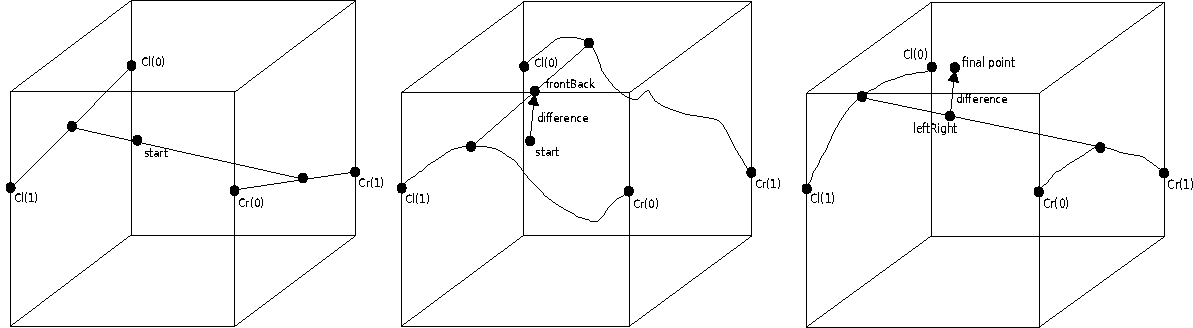
\includegraphics[width=\linewidth]{thesis/layerCreation.pdf}
 \caption{The calculation of a point in the layer grid. First, find the starting point by interpolating the four courners for the current position in the grid. Second, interpolate the front and back curves at the current position, and calculate the difference from the starting point. Third, interpolate the left and right curve at the current position, and finally add the previously calculated difference to this point, yielding the final point}
\end{figure}



The heights in each point of the grid are not a regular height grid, but are heights according to the parametric coordinates along the curves on the side of the cube where the index divided by the resolution gives the parametic coordinate. This fits well with the parametric representation of all features, and makes it easy to associate the parametric coordinates with each point in the grid. It also enables the user to draw curved surfaces without loosing resolution on steep slopes. It also enables the user to draw surfaces that loop back over themselves, that is they do not go strictly from left to right or from right to left. This does mean that some features to be drawn on the surface of the layer later, might not have a well defined behaviour in such areas where the surface does loop back over itself, but it also enables the user to model certain geological fenomena such as folding of layer structures.

Once a grid has been created, each of the features that needs to make modifications get the chance to do so. All features that are drawn on the surface implement an interface that enables the layer object to tell them to do their modifications at the correct time. Each feature does this in the order they were created. How they do this is covered under each of the features explanation below.

For the geometry, triangles are created between the points of the grid. Normals for each vertex is created by averaging the normal of the triangles surrounding the point. Then for each of the sides of the cube another surface is created between the curves of this layer and the layers below.

The sides of the layer is created for each face of the cube by filling the area between the curve of the layer for that face and the topmost point of each of the curves of the layers below. If the current layers curve goes below the layers below, then no fillings are created in the area demarked by this section of the curve. The cube will maintain a curve that represents the top of the layers below, and this will be updated as new layers are added. Therefore the layer itself needs only consern itself with this curve, and not all of the previous layers.

For updating the curve demarking the top of all layers, the following prcedure is used. 
\begin{enumerate}
 \item Create an empty curve newPoints
 \item For each intersection from left to right, a point is created at this intersection. Then check which of the points from each curve preceding the intersection is the topmost. Add all the points from the topmost curve since the last intersection, or if this is the first intersection, since the beginning to newPoints.
 \item At the end add the rest of the points since the last intersection, or if no intersections since the beginning to newPoints, from the topmost curve.
\end{enumerate}

For detecting which areas of a face of the cube to cover with the layers surface polygons are created and then geometry is created from there. This procedure is used:
\begin{enumerate}
 \item Create a list of lists of points, call it ``polygons''
 \item Create a point between the first point of the layer curve and the curve demarking the top of all layers, call it ``previousIntersection''
 \item For each intersection from left to right, create a point ``intersection''. Then add ``previousIntersection'' to a new list of points ``polygon''. Check which of the two curves are the tomost at the point before the intersection. Add all points between the previous intersection and the current intersection from the topmost curve. Add the point ``intersection''. Add, in reverse order, all the points between the current intersection and the previous intersection from the lowermost curve. Add ``polygon'' to the list ``polygons''.
 \item For each polygon in the list ``polygons'', create a triangluation suitable for visualization, and add all triangles to the geometry.
\end{enumerate}

\subsection{Rivers}
Rivers can be drawn on the surfaces by indicating where it will run. The program then creates a river as shown in figure \ref{fig:riverDraw}. It can also be changed by oversketching as shown in figure \ref{fig:riverChange}. The oversketching is done on one side of the river at a time. The user also has the choice of replacing the entire side of the river if that will let him more easily make the changes he wants.

\begin{figure}
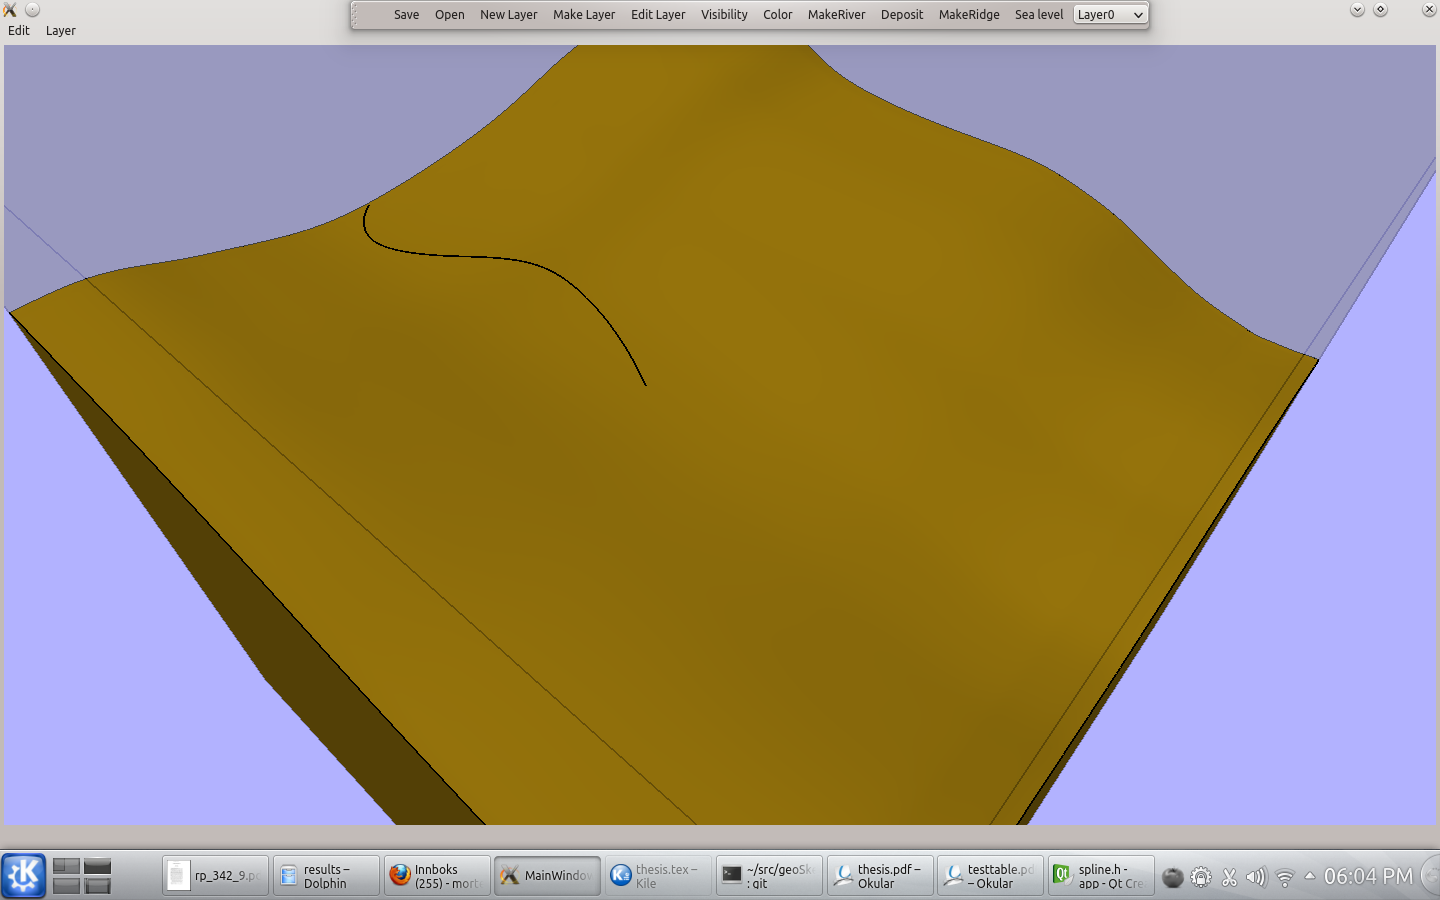
\includegraphics[trim = 30mm 80mm 120mm 30mm, clip,width=.5\linewidth]{thesis/results/riverDraw.png}
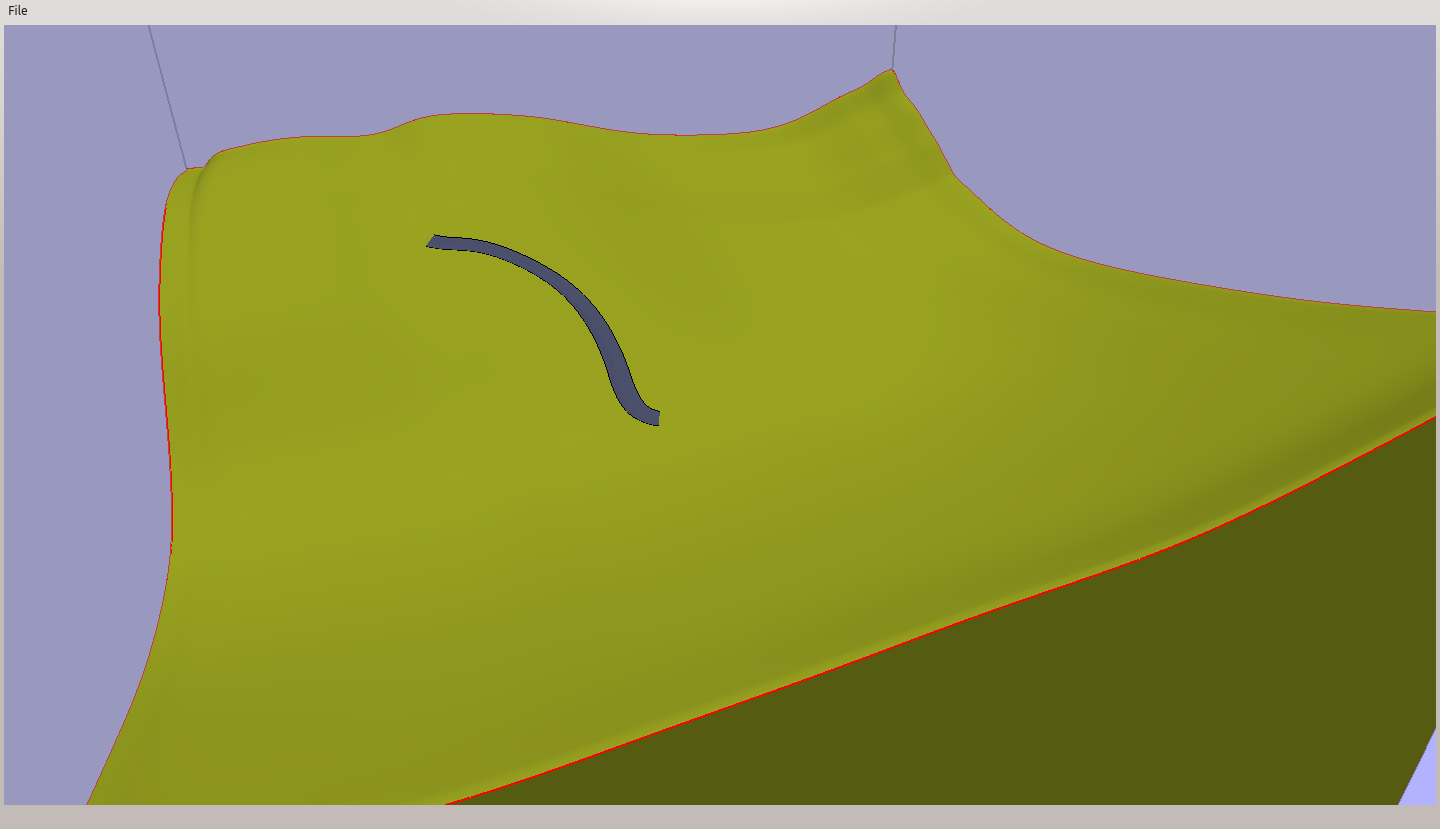
\includegraphics[trim = 30mm 80mm 120mm 30mm, clip,width=.5\linewidth]{thesis/results/riverDrawn.png}
 \caption{Sketching of rivers by indicating where it should run, and letting the program create a river along this path. }
 \label{fig:riverDraw}
\end{figure}

\begin{figure}
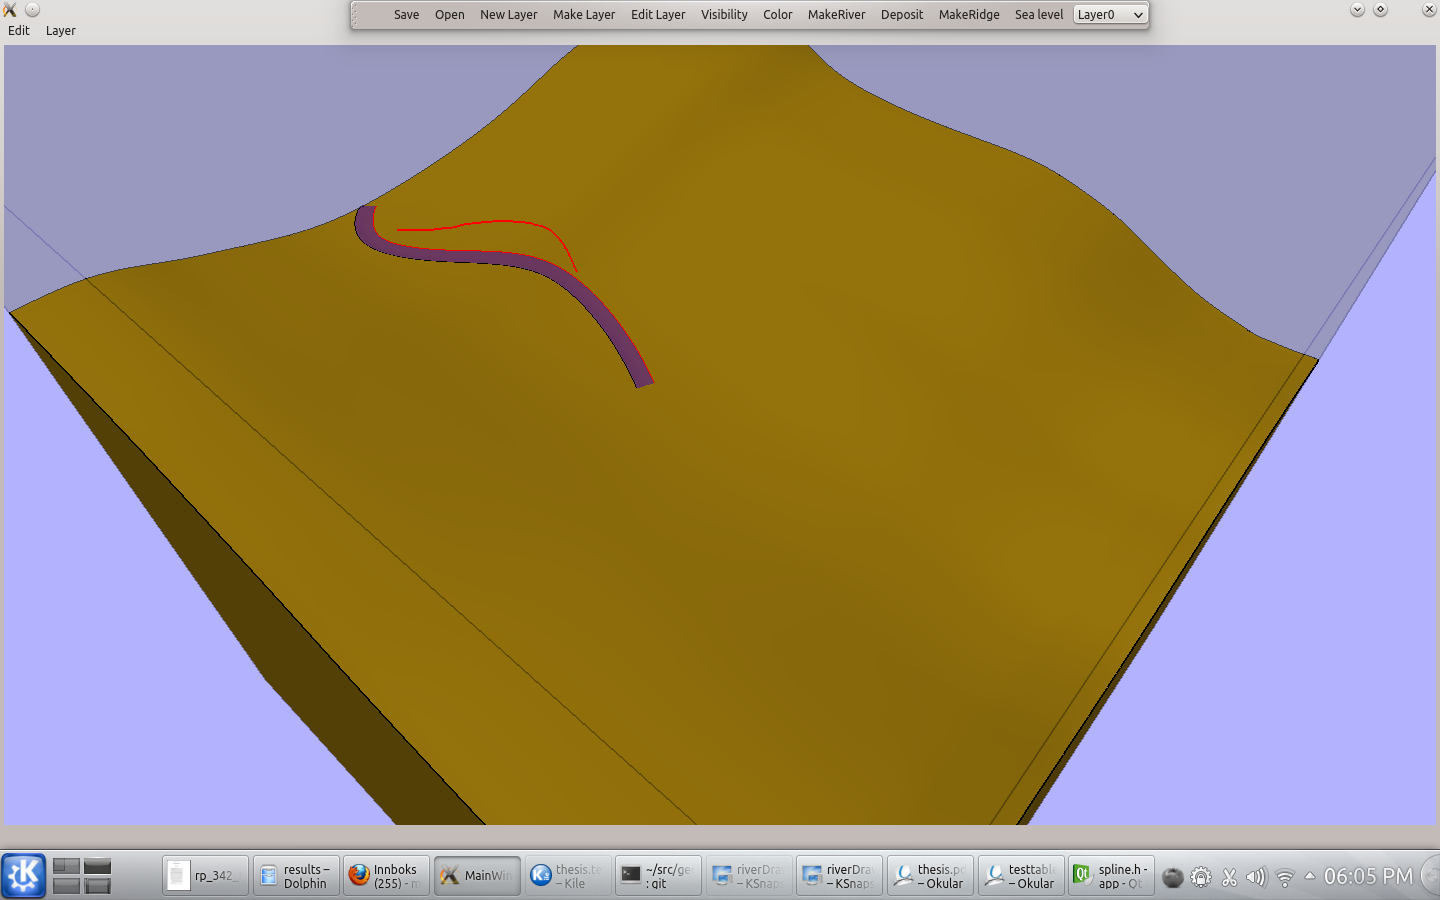
\includegraphics[trim = 30mm 80mm 120mm 30mm, clip,width=.5\linewidth]{thesis/results/riverChange.png}
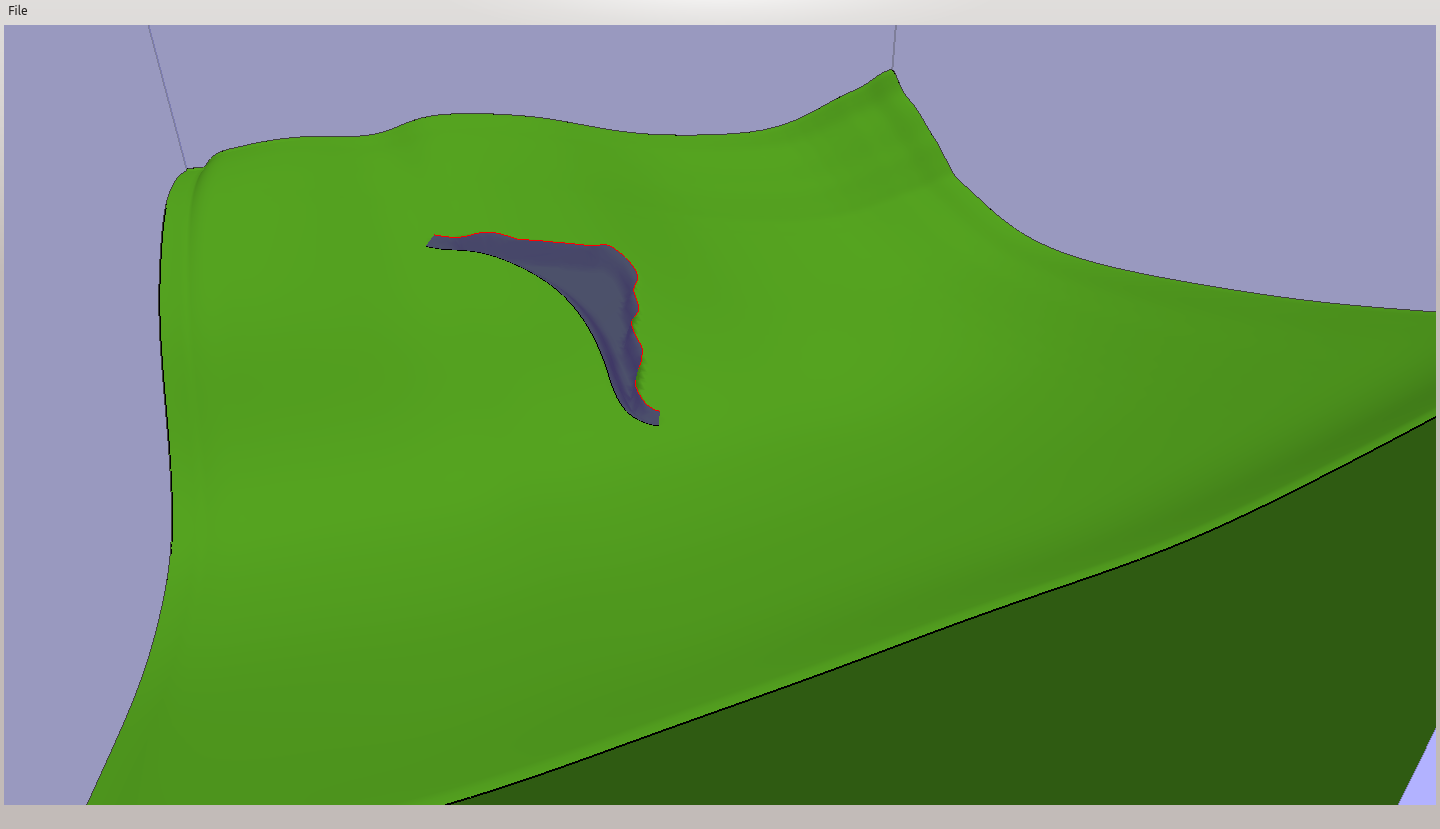
\includegraphics[trim = 30mm 80mm 120mm 30mm, clip,width=.5\linewidth]{thesis/results/riverChanged.png}
 \caption{Changing a river is possible by oversketching }
 \label{fig:riverChange}
\end{figure}


\subsection{Valleys}
A valley functions much like a river, only it has no water and is initally wider and deeper. It is also made by first drawing a line and then can be changed by the same mechanism as the river.
\begin{figure}
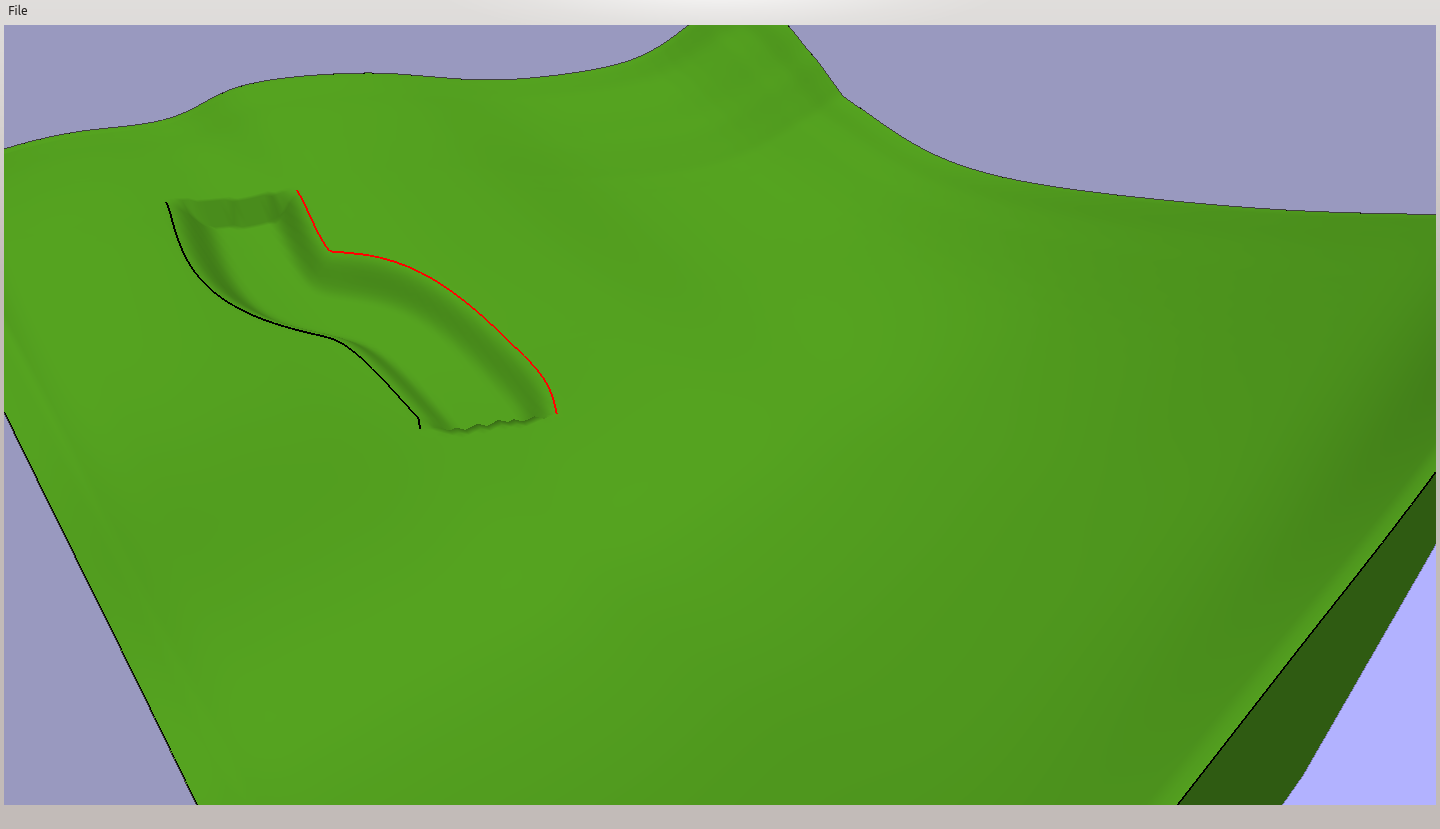
\includegraphics[trim = 10mm 80mm 200mm 30mm, clip,width=.5\linewidth]{thesis/results/valleyMade.png}
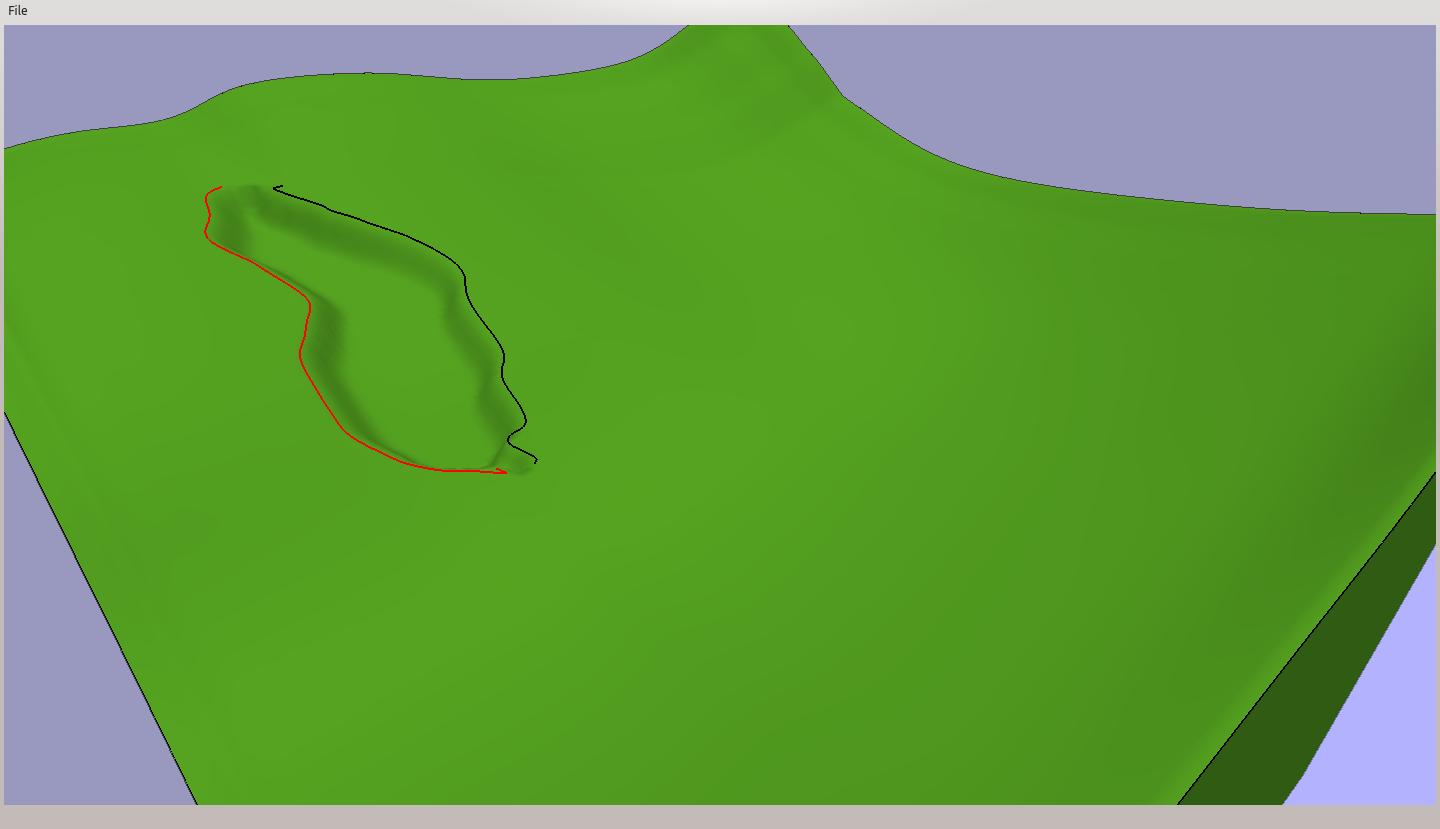
\includegraphics[trim = 10mm 80mm 200mm 30mm, clip,width=.5\linewidth]{thesis/results/valleyChanged.png}
 \caption{A valley and the same valley after a change to both of it's sides }
 \label{fig:valley}
\end{figure}

\subsection{Ridges}
Ridges are also drawn by a line on the layer surface. Once a line has been drawn and the user indicates that he want's a ridge, a generic shape of a ridge is created automatically as seen in figure \ref{fig:ridgeDraw}. The user then has the choice to change the height profile along the ridge's baseline. This is done by skething on a temporary wall that is erected along the ridge's baseline, as can be seen in \ref{fig:ridgeChange}

\begin{figure}
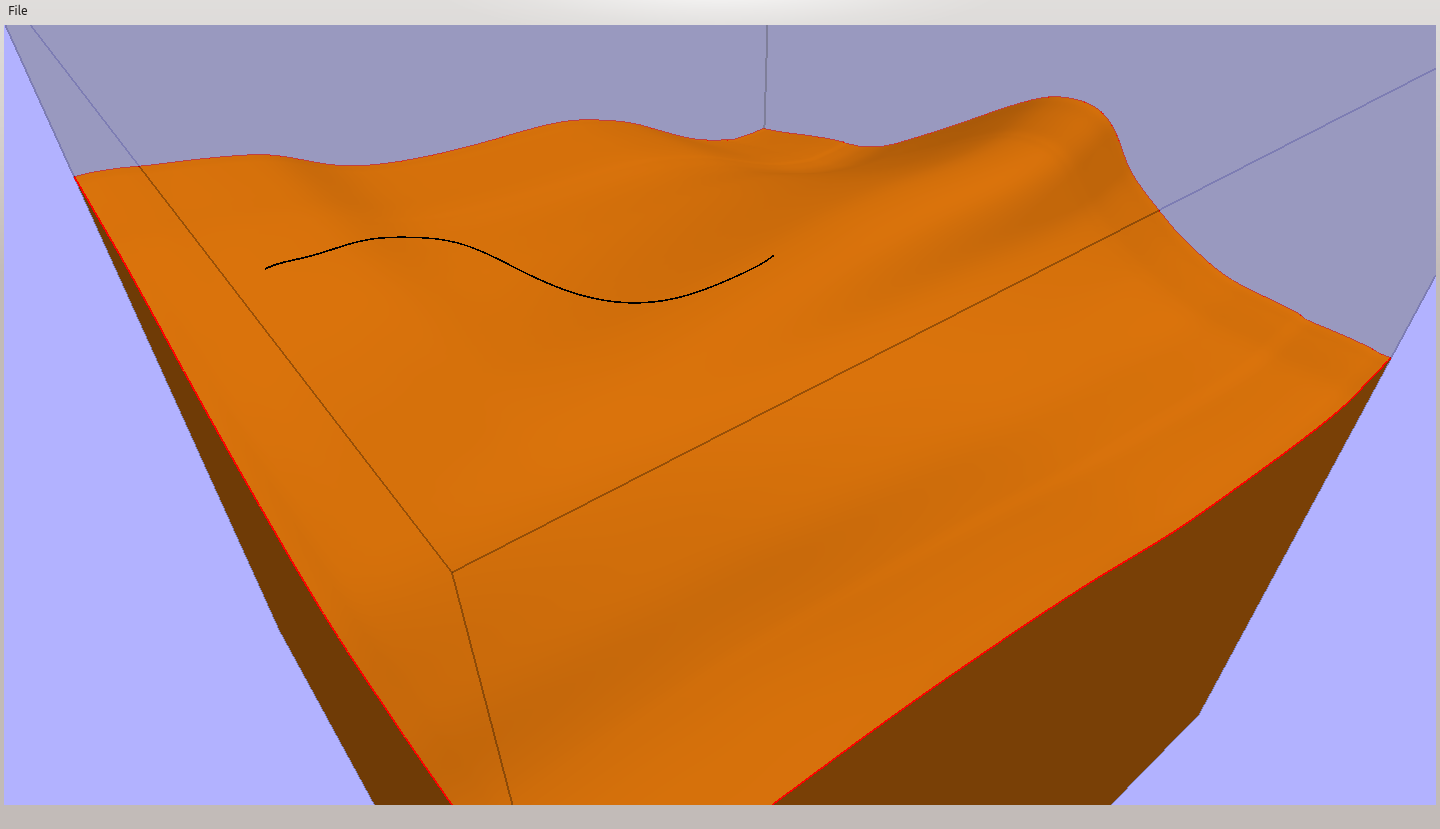
\includegraphics[trim = 30mm 80mm 120mm 30mm, clip,width=.5\linewidth]{thesis/results/ridgeDraw.png}
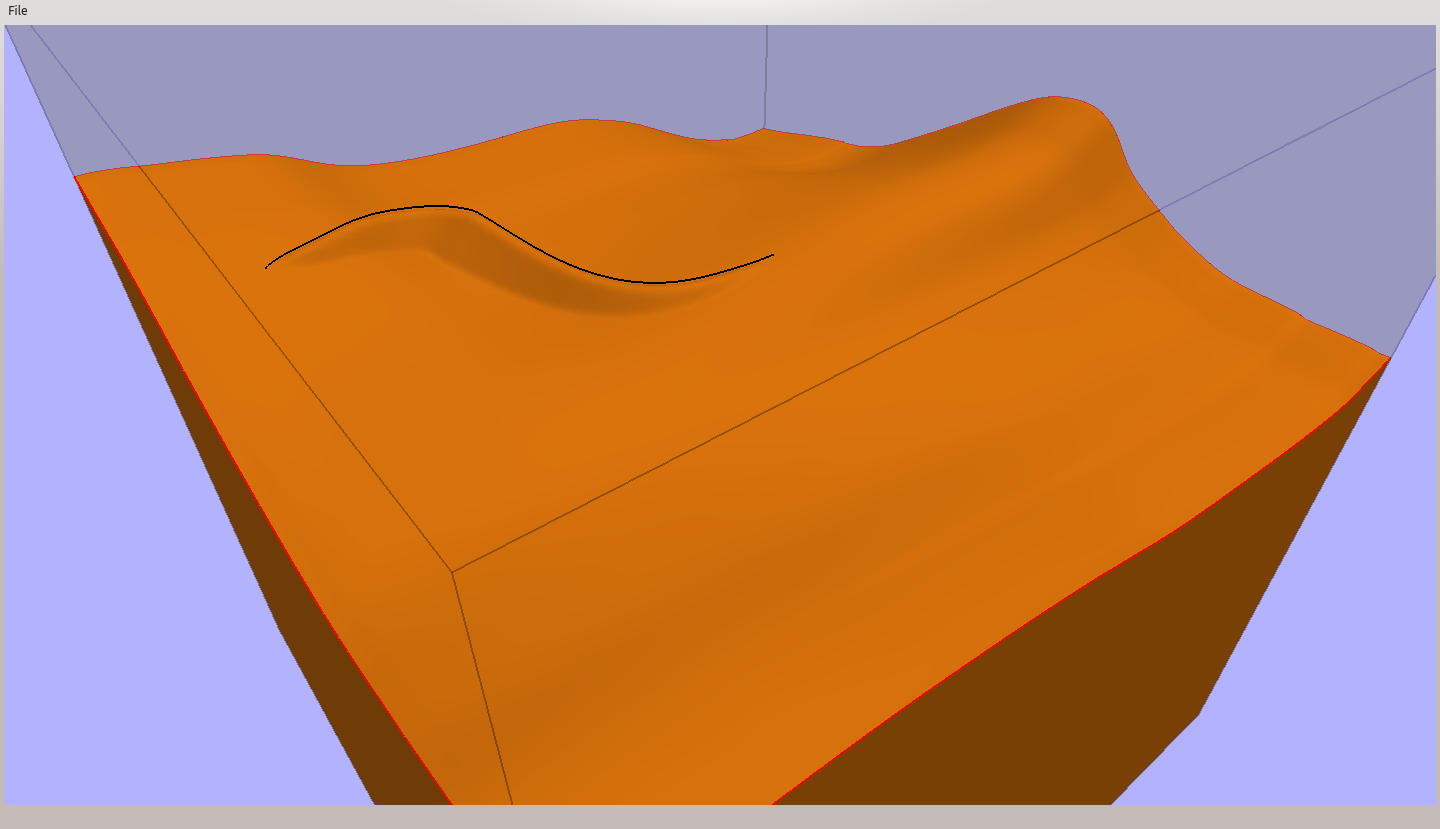
\includegraphics[trim = 30mm 80mm 120mm 30mm, clip,width=.5\linewidth]{thesis/results/ridgeDrawn.png}
 \caption{Sketching of a ridge by indicating where it's base goes, and letting the program create a ridge along this path. }
 \label{fig:ridgeDraw}
\end{figure}

\begin{figure}
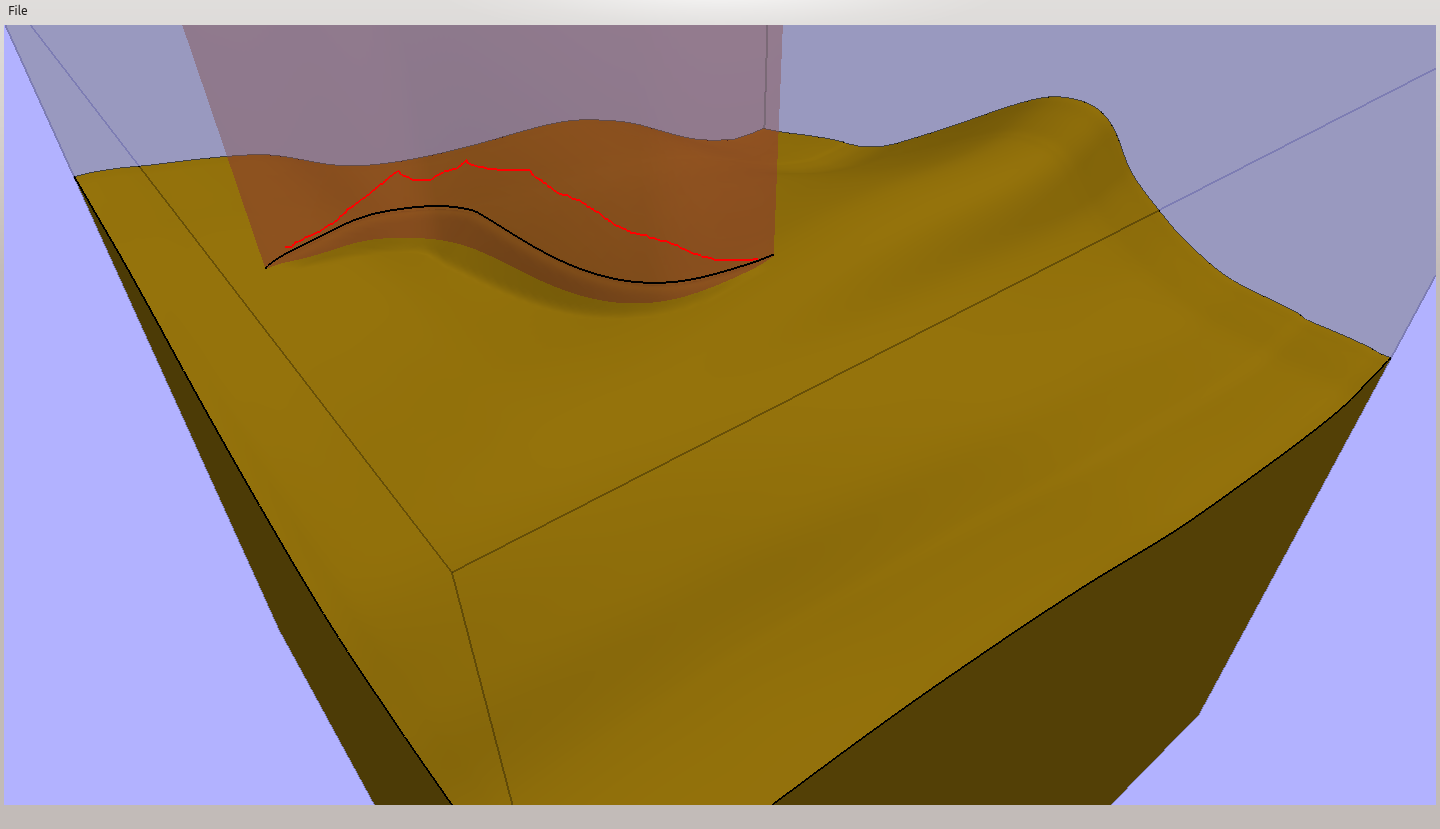
\includegraphics[trim = 30mm 80mm 120mm 30mm, clip,width=.5\linewidth]{thesis/results/ridgeChange.png}
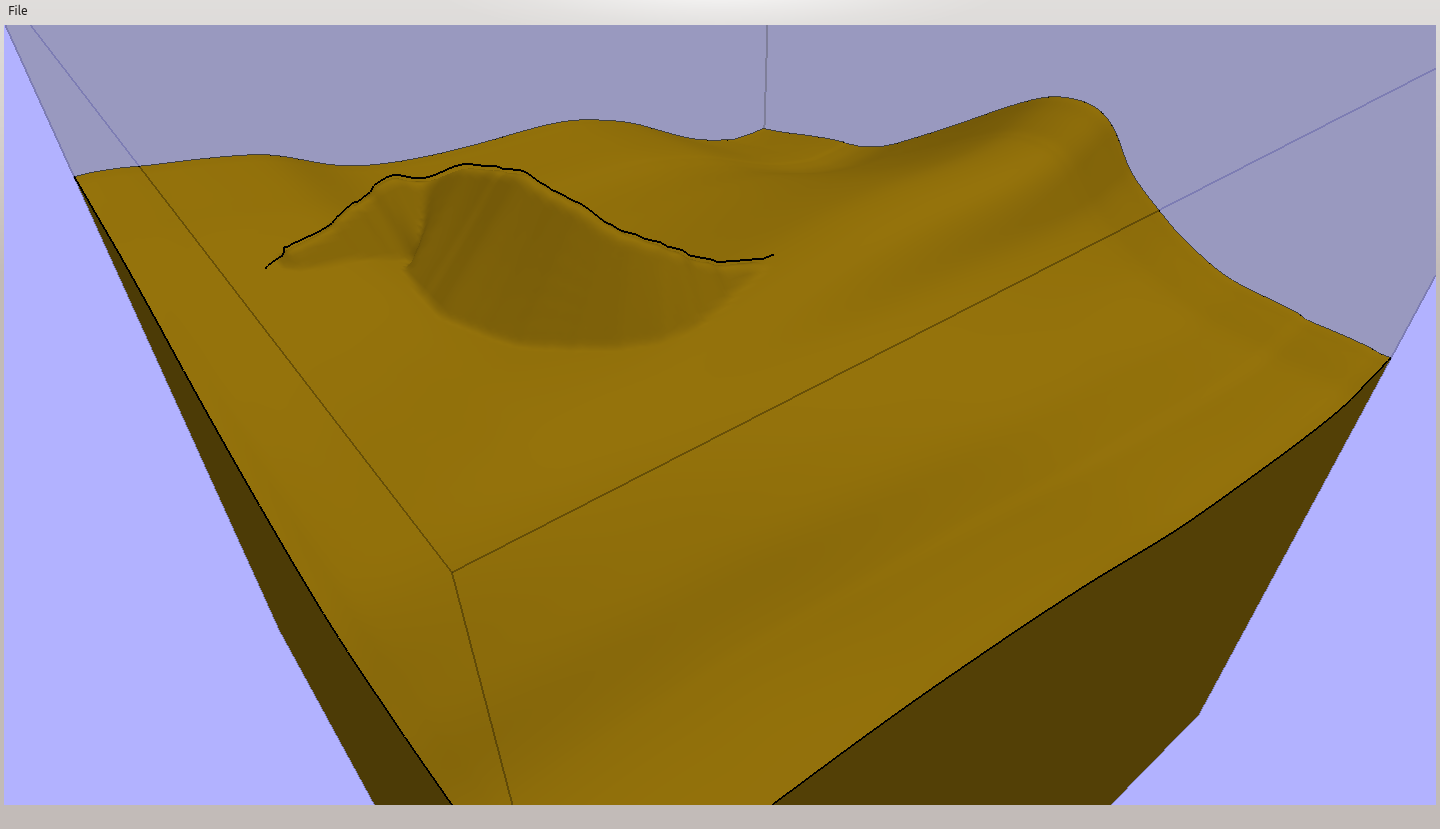
\includegraphics[trim = 30mm 80mm 120mm 30mm, clip,width=.5\linewidth]{thesis/results/ridgeChanged.png}
 \caption{Changing a ridge is done by drawing on a wall that is erected along the ridge's baseline. }
 \label{fig:ridgeChange}
\end{figure}


Input for the ridges is first drawn on a layer as a normal curve. When the user indicates that he wants to create a ridge, a new ridge object is created based on this. A ridge is represented by this curve and a height associated with each point in the curve. The curve is the base line that the user drew on the layer where he wants the ridge to follow along. The heights are the height of the ridge at each point of the curve. Initially the height list is just a smooth function from side to side of the ridge, with a peak in the middle. The height can be changed if the user indicates so. This new height line is input on a temporary sketch wall erected for this purpose. The input prcedure is similar to other lines, but in the end it is not actually stored as normal line. When the user is done, only the height along the entire wall is stored in a list, one for each point on the base line. The wall is constructed by vertices with parametric coordinates that make it easy to read the height from each intersection, as 
well as where along the curve each point is. If the user inputs a line that does not go strictly from left to right or right to left, but loops back over itself, only the last input for that position will be relevant as it will overwrite the former height stored there.

The ridge object itself is visualized only by a curve along the top of the ridge. This is constructed by iterating along the points of the base line. For each point in the base line, the corresponding three dimentional point is found by looking up this point on the layer the ridge belongs to, that is it's parent. Afterwards the height of this point is simply increased based on the relevant height in the list. This yields a new list of points which can then be used to draw a line on screen.

The sketch wall is a simple transparent wall made of triangles between the base line and a set height above it.

*** Rivers and Valleys
Rivers and valleys are represented using two lines, one for each bank of the river or each side of the valley. These lines are constructed based on an initial line input by the user. The original line is then discarded. 


\subsection{Deposits}
Deposits can be created where a river meets the sea. The user simply indicates that he want't one for a river, and the rest is done procedurally by a simple simulation. The procedure continues until the user stops it. The user can indicate more than one deposit to be made for a single river. This will make the deposits build outward on top of each other in the direction of the river.

\begin{figure}
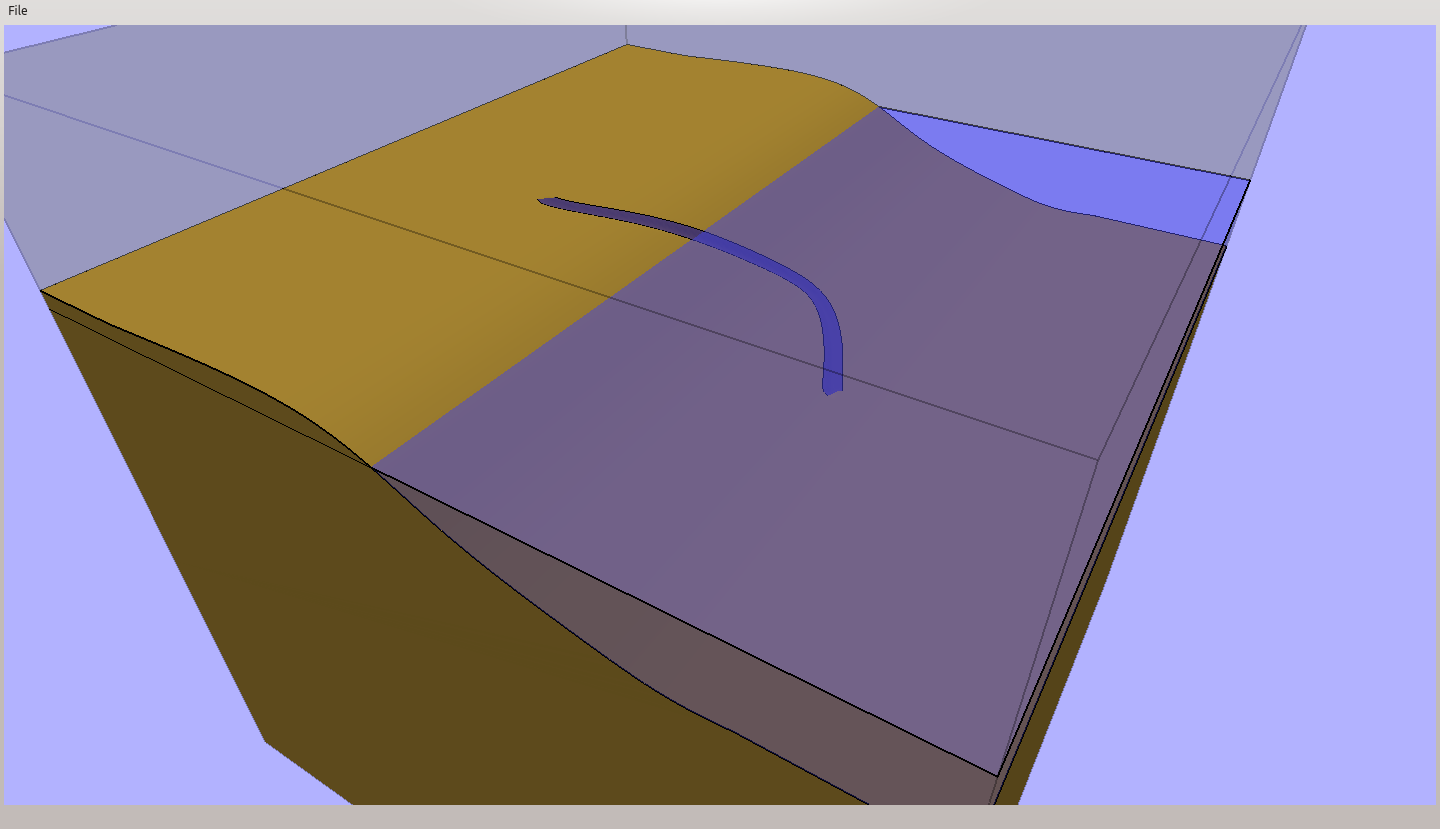
\includegraphics[trim = 90mm 7mm 80mm 30mm, clip,width=.5\linewidth]{thesis/results/depositBefore.png}
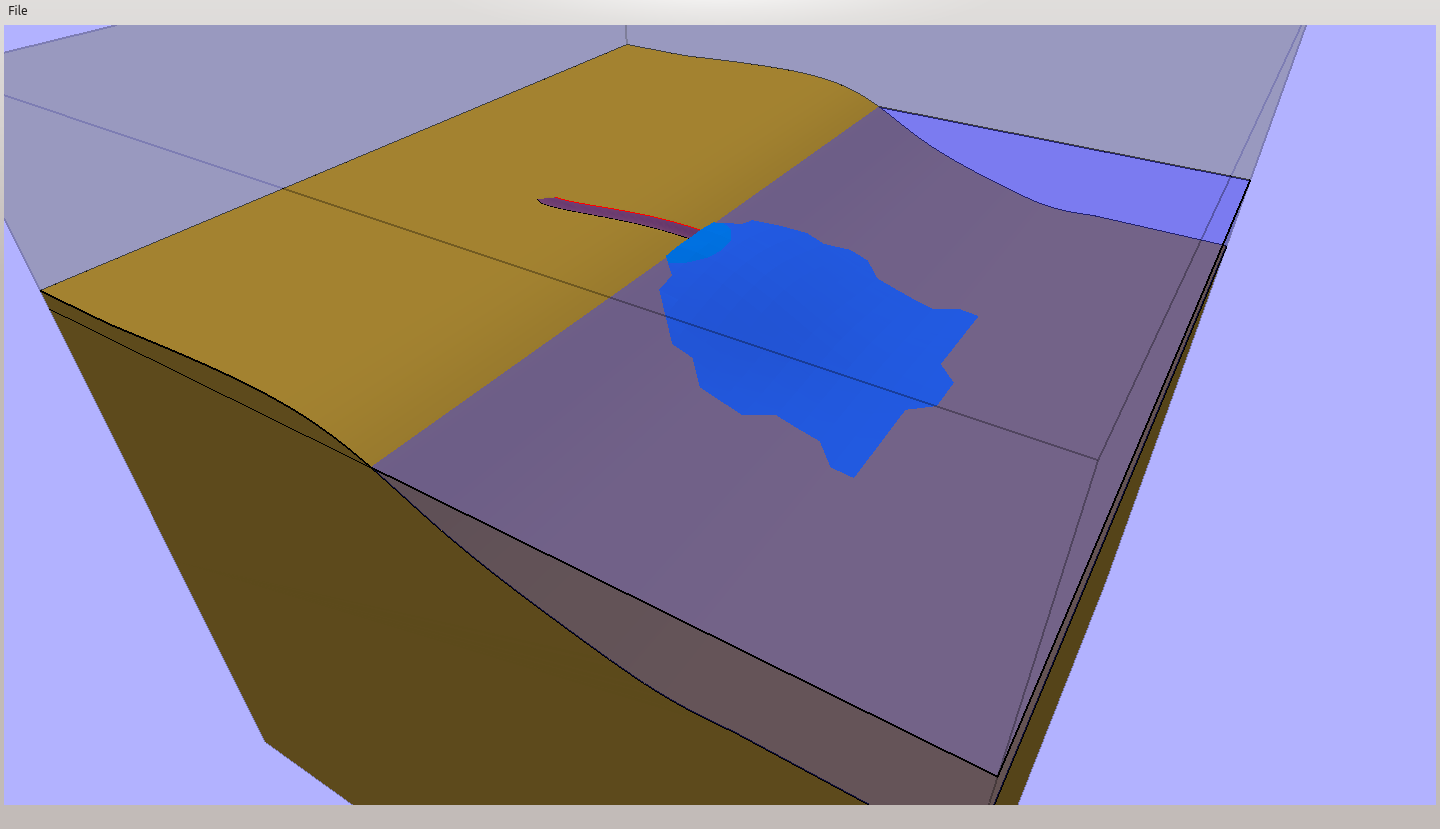
\includegraphics[trim = 90mm 7mm 80mm 30mm, clip,width=.5\linewidth]{thesis/results/depositCreated.png}
 \caption{Creation of a deposit is done procedurally from the point where the river meets the sea}
 \label{fig:depositCreate}
\end{figure}


\begin{figure}
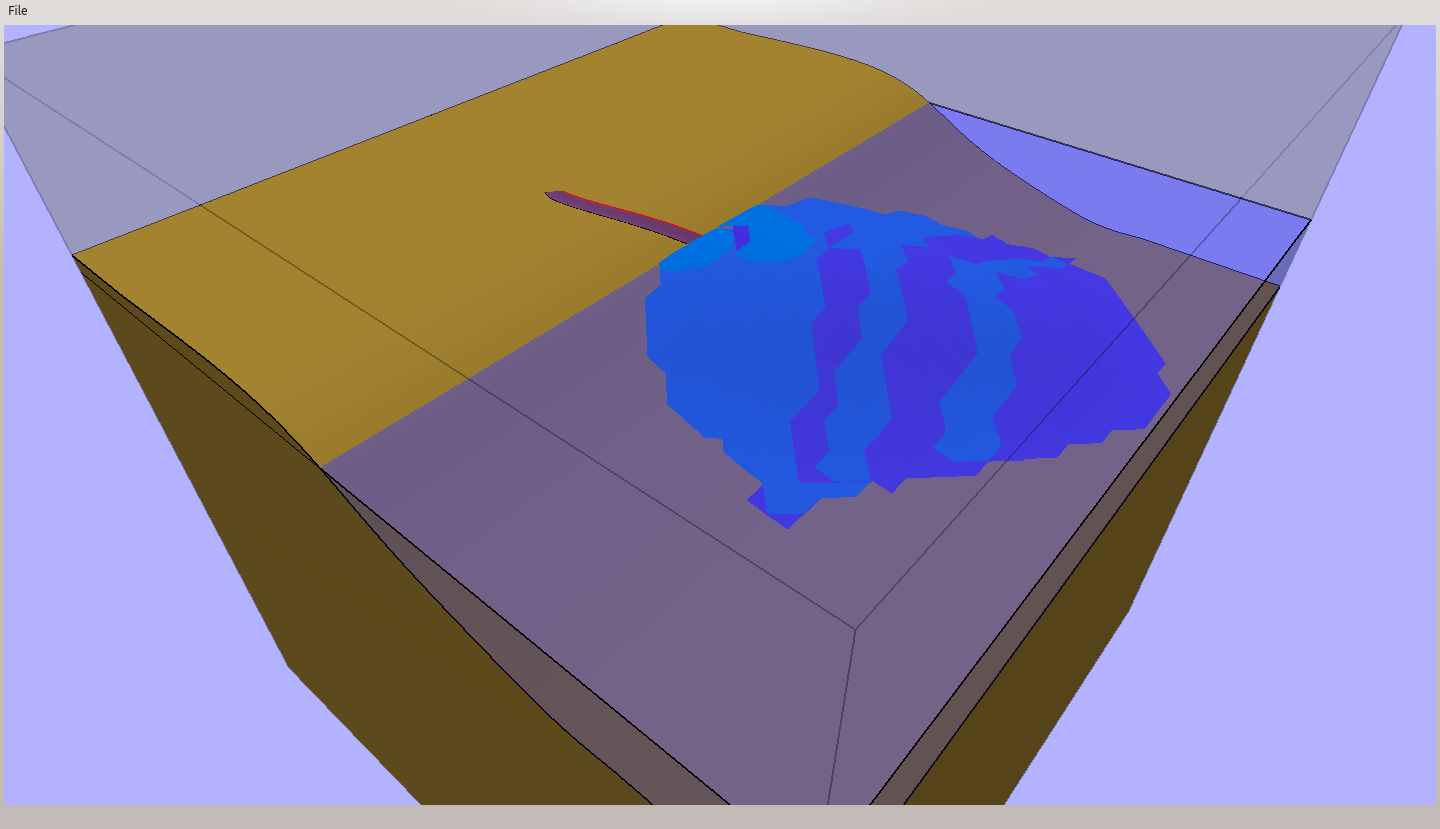
\includegraphics[trim = 120mm 7mm 30mm 30mm, clip,width=.5\linewidth]{thesis/results/depositLayered.png}
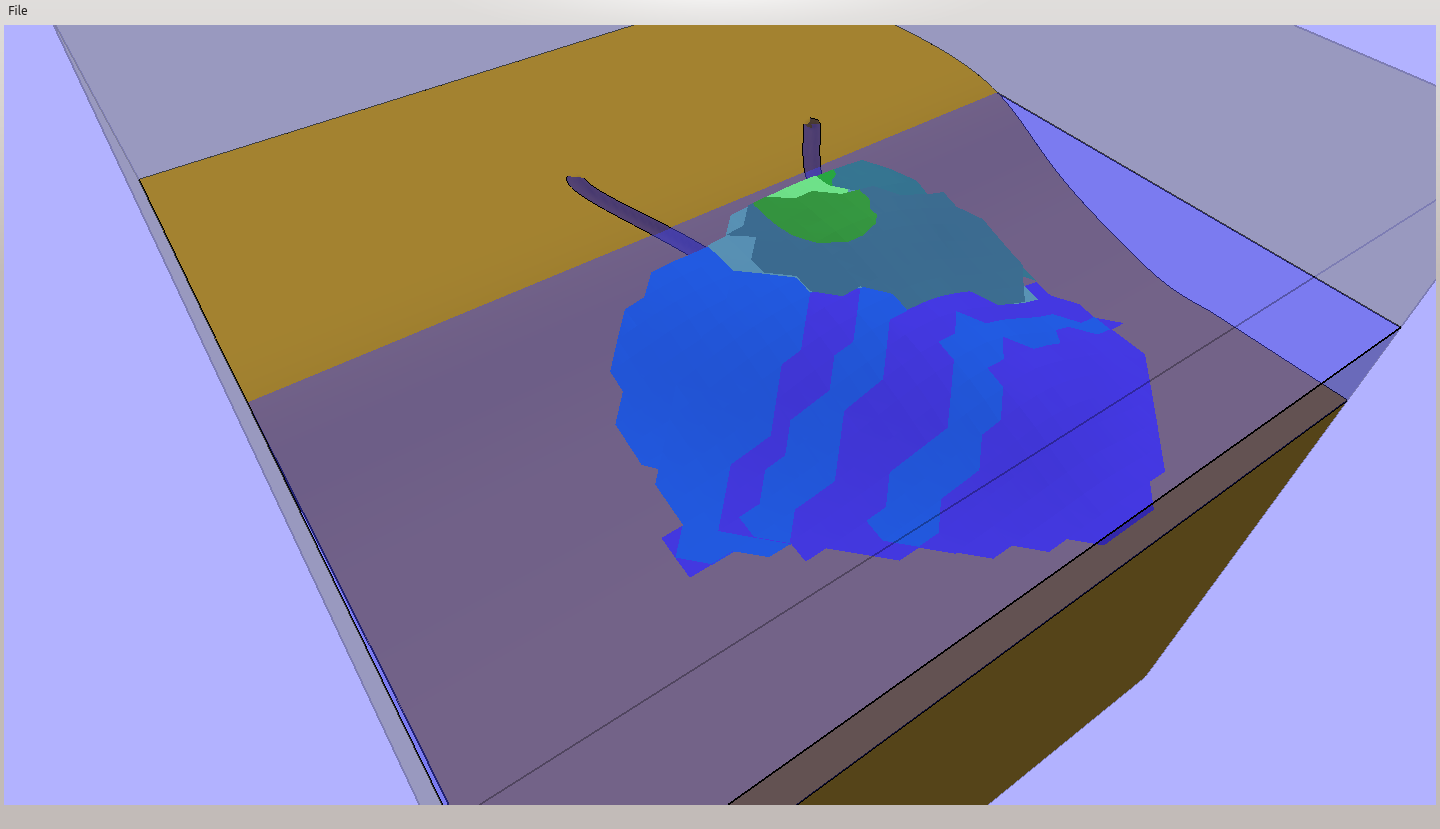
\includegraphics[trim = 120mm 7mm 30mm 30mm, clip,width=.5\linewidth]{thesis/results/depositNew.png}
 \caption{The user can indicate when he wants a new layer of deposits, or when he want's to stop depositing. He can also add new rivers with new deposits.}
 \label{fig:depositLayer}
\end{figure}


Deposits are created procedurally. Therefore, the input for a deposit is implied by the river that the deposit is flowing from and where that river goes below the sea level at the time when the user requests a deposit be made and how long he wishes to let it continue depositing. Deposits are represented by the position where they start, a little below the point in the river where the sea starts, and the amount of matter that is deposited from this point over time. The intention was to also take into account the direction and speed of flow in the river, but this has not been implemented yet.

Since the river is created procedurally over time, it needs an additional step to generate an intermediate representation of the deposit before generating geometry. This step consists of simulating the flow of matter across the surface underneath. For the simulation a simple volume preserving diffusion algorithm is used, that is a modified version of the one found in (??? REFER to webgl flow thing???). This algorithm assumes a regular height grid, and all the underlying layers mut be taken into account. The layers are of course represented as a irregual grid and thus a sampling must be performed to create a regular grid. First a grid overlay over the cube is created at the desired resolution and each point in the grid is set to a value low enough that no intersection could occur at this height. Then at regualar intervals, a ray is cast directly down into the cube, doing intersection tests for each layer, updating the grid value to the height of any intersection when that intersection is higher than the 
current value.

When the height grid is ready, the simulation can begin. The simulation uses an additional grid, to keep track of the amount of deposits at each point. Here follows a description of the simulation algorithm ( see algorithm \ref{alg:layer} for pseudocode );
1. Some matter is deposited at the point where the deposit starts (where the river meets the sea), such that is does not go above the sea level. A variable keeps track of how much has been deposited over time.
2. For each axis in the grid(x direction and y direction), for each point in the grid;
Set the deposit height of the current cell to it's previous value plus half the difference as compared to the previous cell (according to the axis currently considered and the next cell. Both these values are clamped by the available amount of matter. The algorithm is given as pseudocode in \ref{alg:layer}


\begin{algorithm}
\caption{Pseudocode of the deposit simulation algorithm. Let the current cell be denoted as C(i,j) the previous value of the cell $P(i,j)$, the terraint height $T(i,j)$ and the axis vector $A(i)$ is either $x = (1, 0)$ or $y = (0, 1)$, and a flow rate function $F(i,j) = 2 + M(i-A(0, j-A(1)) ^{flowRate}$ where flowrate is a number between 1 and 2 as chosen by the user. The new value for each cell is then computed as follows:}
\label{alg:layer}
\begin{algorithmic}
    \For{$A = x, y$}
      \State $left \gets (i,j)-A$
      \State $rigth \gets (i,j)+A$
      \State $tl \gets T(left)$
      \State $dl \gets P(left)$
      \State $tr \gets T(rigth)$
      \State $dr \gets P(rigth)$
      \State $diffLeft \gets (tl+dl) - (T(i,j) + P(i,j))$
      \State $diffRigth \gets (tr+dr) - (T(i,j) + P(i,j))$
      \State $flowLeft \gets clamp (diffLeft/F(left), -d/2, dl/2)$
      \State $flowRigth \gets clamp (diffRigth/F(rigth), -d/2, dr/2)$
      \State $C(i,j) \gets P(i,j) + flowLeft + flowRigth$
      \If{$flowLeft > 0 \And M(left) + 1 < M(i,j)$}
	 \State $M(i,j) \gets M(left) + 1$
      \EndIf
      \If{$flowRigth > 0 \And M(rigth) + 1 < M(i,j)$}
	 \State $M(i,j) \gets M(rigth) + 1$
      \EndIf
    \EndFor
      
\end{algorithmic}
\end{algorithm}
      
The simulation runs until the user is satisfied and stops it or if the deposit is a preexisting one, until the target deposit amount has been reached. The total amount of deposited matter is stored in the target variable when the user stops the simulation.

Geometry is generated based on the height of the deposits and underlying terrain. When generating geometry special care needs to be given to the orientation of the triangles to give a uniform and smooth look to the visualization. For each column i and row j in the deposit grid, triangles are generated according to the algorith in algorithm \ref{alg:triangle}. 

\begin{algorithm}

 \caption{Triange orientation decicion. D(i,j) is the deposit amount, T(i,j) is the terrain height. A threshold t is used to decide where to draw triangles and where not.}
 \label{alg:triangle}
 \begin{algorithmic}
 
 \For{$j = 0 \to gridsize -2$}
 \For{$i = 0 \to gridsize -2$}
  \State $a \gets (i,j)$
  \State $b \gets (i,j+1)$
  \State $c \gets (i+1,j)$
  \State $d \gets (i+1, j+1)$
  \If {$D(c) > t \And D(b) > t$}
     \If {$D(a) > t$}
	\State create triangle between a, b, and c
     \EndIf
     \If {$D(d) > t$}
	\State create triangle between b, d, and c
     \EndIf
  \ElsIf {$D(a) > t \And D(d) > t$}
     \If {$D(b) > t$}
	\State create triangle between a, b, and d
     \EndIf
     \If {$D(c) > t$}
	\State create triangle between a, d, and c
     \EndIf
  \EndIf
  \EndFor
  
  \EndFor
  
 \end{algorithmic}

\end{algorithm}


  
This algorithm in gives triangles that follow the entire outline of the deposit smoothly, where a naive approach always gives jagged edges at one side and smooth edges at the other side.

\begin{figure}
 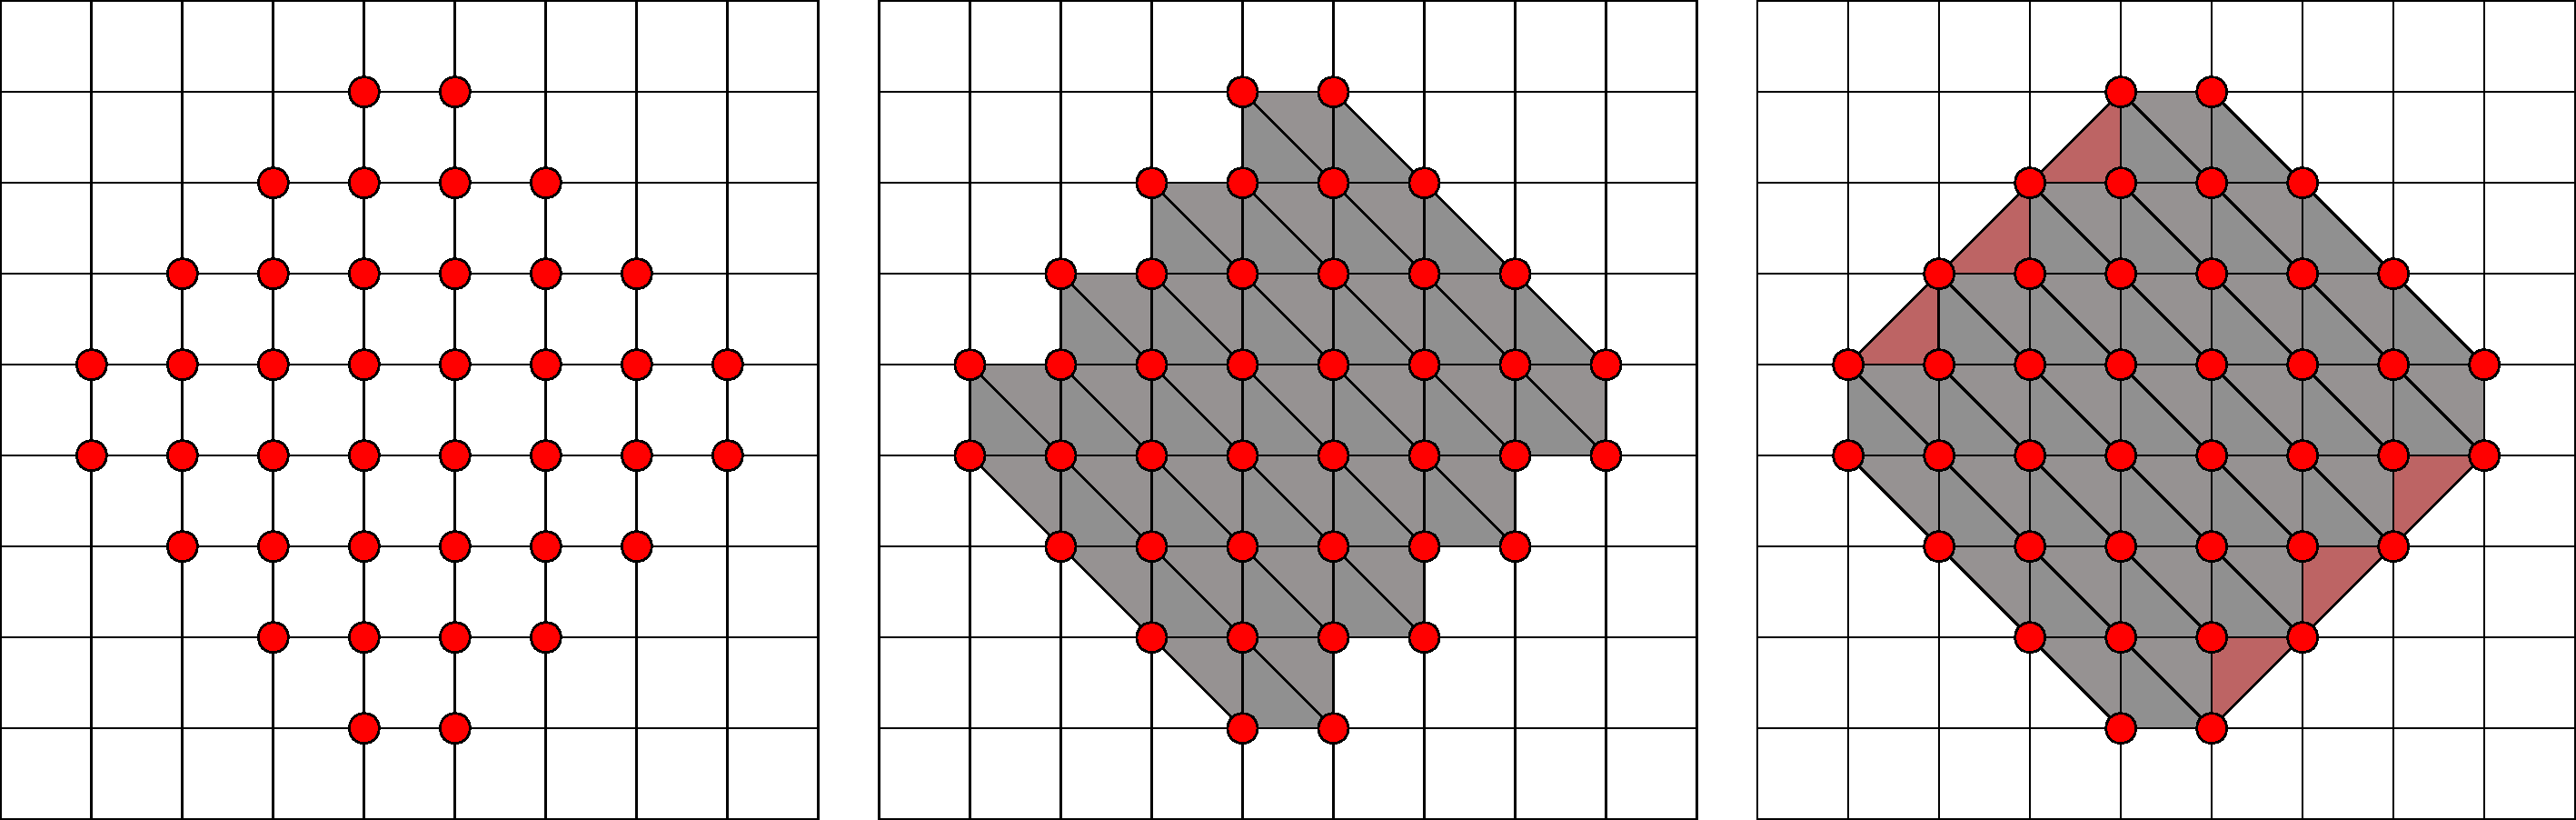
\includegraphics[width=\linewidth]{thesis/gridtrianglesall.pdf}
 \caption{Triangle orientation. Left; the grid points that have matter deposits above the threshold. Middle; the first, naíve approach where all triangles are oriented the same direction. Right; the more sophisticated approach, where the triangle orientation depends on which surrounding points have deposited matter. As seen on this illustration, the second approach gives a more uniform look on each side of the structure, while the first approach gives more jagged edges and non-uniform look}
\end{figure}


When creating a deposit, the layer object will check for previous deposits, and if such exists, the grid data will be reused for the next deposit. This gives not only speed improvement, but also enebles deposits to flow on top of each other.

\subsection{Sea level}
The sea level can be enabled at any time and moved up or down as the user pleases. Where a river meets the sea, a deposit may be generated.

\begin{figure}
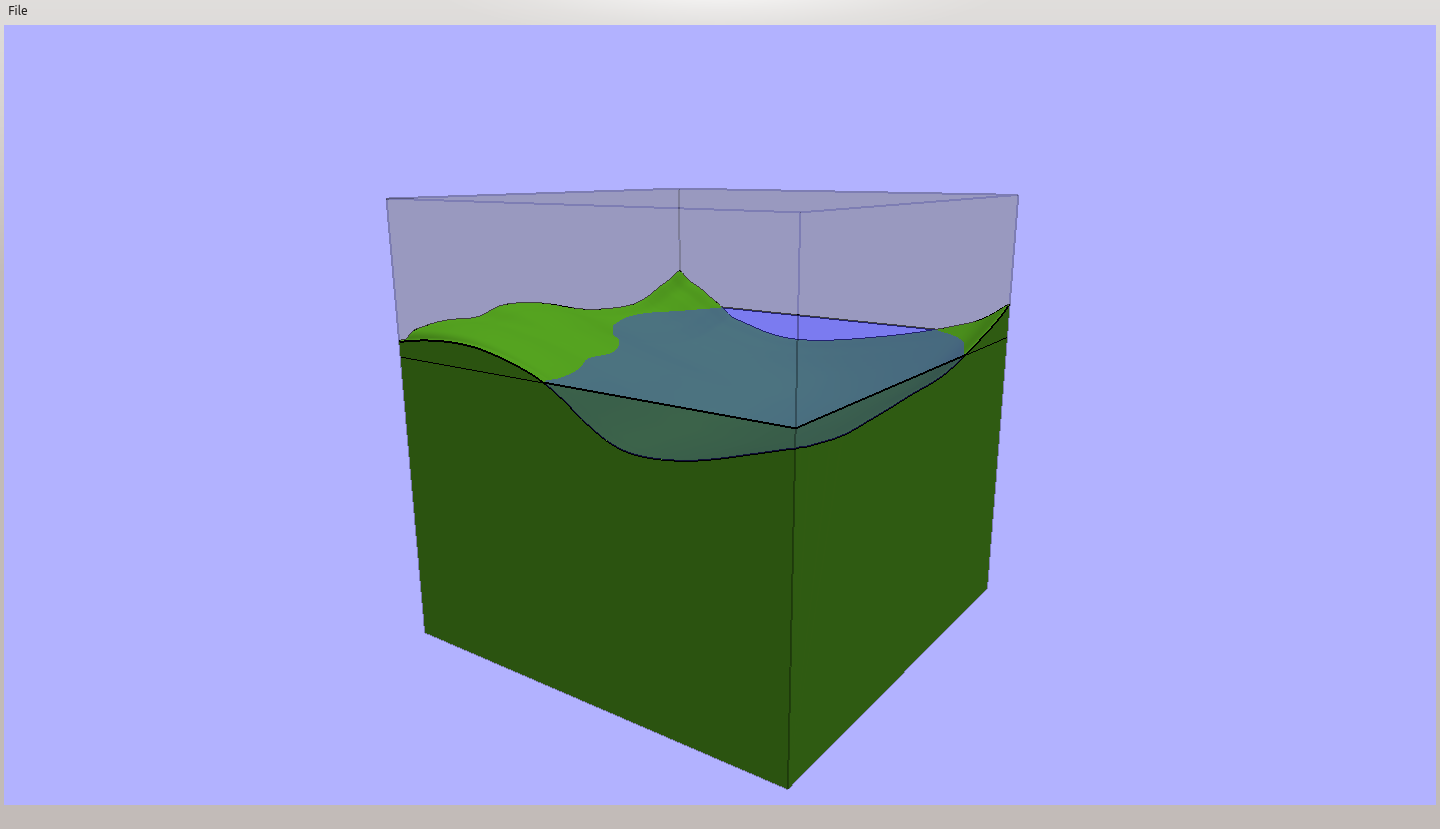
\includegraphics[trim = 90mm 7mm 80mm 30mm, clip,width=.5\linewidth]{thesis/results/seaEnabled.png}
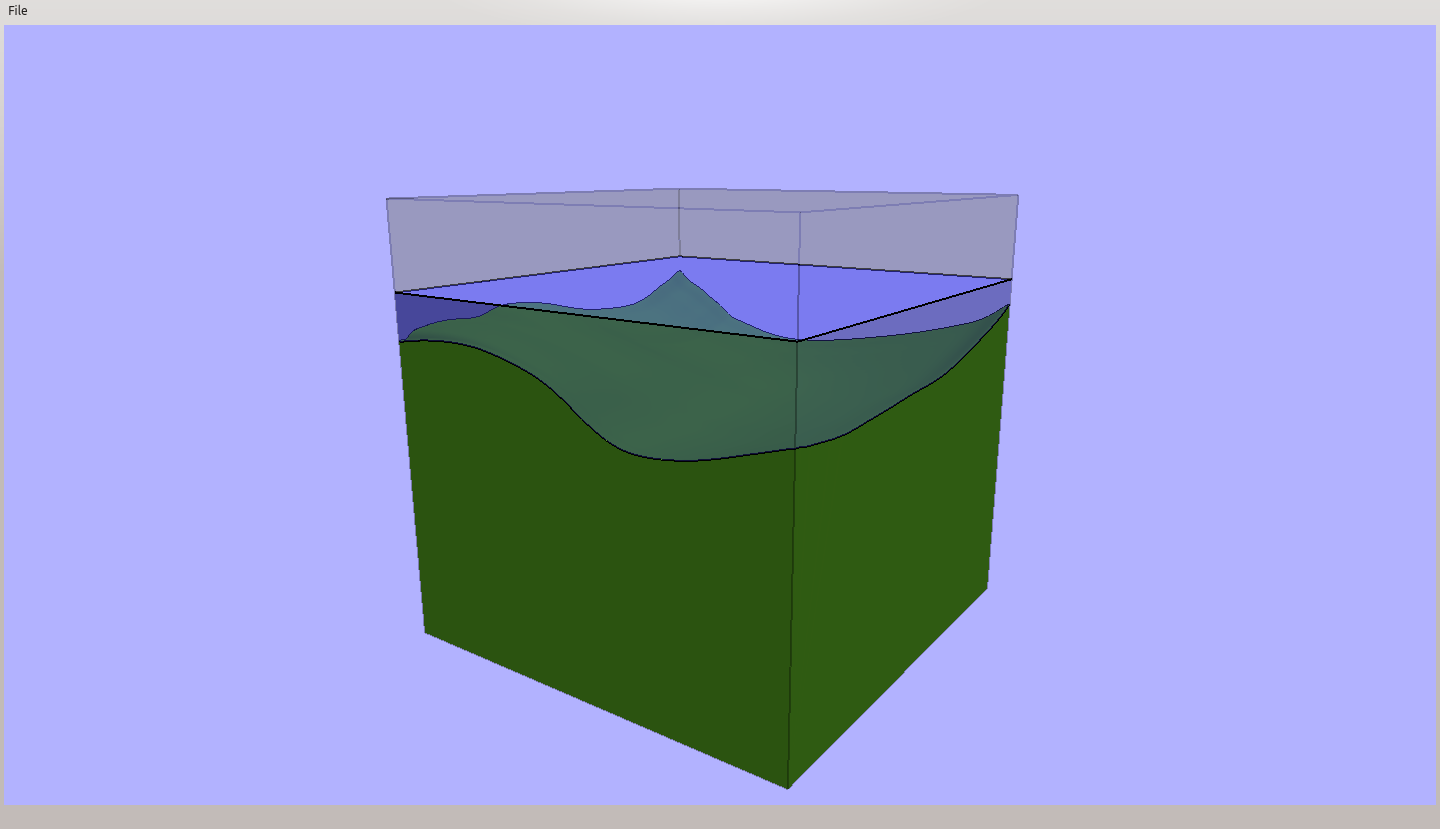
\includegraphics[trim = 90mm 7mm 80mm 30mm, clip,width=.5\linewidth]{thesis/results/seaChanged.png}
 \caption{Indicating where the sea level goes}
 \label{fig:seaLevel}
\end{figure}


\clearpage
\chapter{Results}
Here we will see some complete sceneries that demonstrate what can actually be produced by the implemented solutions at the current level of development. These results are commented to explain how they are achieved, what they depict and what are the limitations. Then we will take a look at the results of a user study that was conducted. An evaluation of the results follows in the next section.
\label{sec:results}

\section{Scenarios}


\section{Produced Renderings}
\subsection{Geologist's drawings}
- Marie might draw her stuff?
\subsection{Reproduction of initial illustrations}
- compare with goal\\
\subsection{Other illustrations and possibilities}

\clearpage
\chapter{Evaluation}
\label{sec:eval}
The test user was often observed to struggle with understanding how the interface works and what the programmer intended him to do to complete a specific goal. It was difficult for the user to put into words what the problem was, and often the problem was that he did not have the knowledge or languag required to communicate it. Observation of user interaction therefore helped in revealing problem areas. Once identified, intelligent questions by a person familiar with the program might help, but what seemed to work better was to try and deduce what the problem could be, propose a solution, first by explanation and later by actually implementing it, and let the user evaluate the new approach.


- learning\\
- usability
 -- (focus on expressiveness) -- \\
- How well problem was solved\\
- Where it will be used \\
- Discussion

\clearpage
\chapter{Conclusion}
\label{sec:conclusion}
- Give short summary\\
- Further work\\
\\


Testing references: Cherlin ~\cite{Cherlin:2005:SMF:1090122.1090145} explores techniques for rapid sketch based 3d modeling.


\bibliography{thesis}{}
\bibliographystyle{plain}
\end{document}
